\documentclass[../thesis.tex]{subfiles}
% \graphicspath{{\subfix{../images/}}}


\usepackage{bm}
\usepackage{natbib}
\usepackage{pdflscape}
\usepackage{afterpage}

\newtheorem{theorem}{Theorem}
\newtheorem{assumption}{Assumption}

% modification to natbib citations
\setcitestyle{authoryear,round,citesep={;},aysep={,},yysep={;}}

% My math notation
% \newcommand{\myscal}[1]{#1}
% \newcommand{\myvect}[1]{\bm{#1}}
% \newcommand{\myrv}[1]{\MakeUppercase{#1}}
% \newcommand{\mycnt}[1]{#1}
% \newcommand{\mydim}[1]{{d_{\MakeUppercase{#1}}}}
% \newcommand{\myfunc}[1]{#1}
% \newcommand{\mylik}[1]{\mathrm{\MakeUppercase{#1}}}
% \newcommand{\myexp}[3]{\mathbb{E}^{\mylik{#1}}_{#2 \sim #3}}

% \newcommand{\crit}[1]{\textcolor{red}{#1}}
% \newcommand{\draft}[1]{\textcolor{blue}{#1}}
\newcommand{\ind}{\perp\!\!\!\!\perp} 
\newcommand{\fzero}{F\textsubscript{0}}

\begin{document}

\chapter{Missing data imputation}

\paragraph{Abstract.} I present a method for applying the group-instance model to the problem of \textit{missing data imputation}. This task aims to infer values for the set of missing instances of an incomplete observation-group in a way that is consistent with the visible instances. I am considering a specific formulation of missing data imputation where the training data comprises only complete observation-groups while the testing observation-groups are incomplete. Moreover, the testing \textit{patterns of missingness} (i.e., which instances of the testing observation-groups are visible and which are missing) are unknown. I call this formulation, \textit{versatile imputation}. Although this formulation is rarely studied in the statistical literature on missing data imputation, it is encountered frequently in real-world applications of imputation with deep learning. The unique challenge of this formulation is the lack of prior knowledge about what patterns of missingness will be encountered during testing. Existing methods generalise poorly across different patterns of missingness so researchers typically design imputation algorithms for specific patterns. By contrast, I propose a method, the \textit{Multiple-Instance Variational Autoencoder} (MIVAE), that can perform imputation across a wider range of patterns. MIVAE is an implementation of the group-instance model where we treat the observation-group itself as a group with the individual instances playing the role of instances. I evaluate this method on the imputation task of \textit{prosody control}, and show that it outperforms the current state-of-the-art model, the masked autoencoder, on a range of patterns of missingness encountered in the literature. Lastly, I discuss a possible theoretical explanation for the improved perfomance brought by my method.

\section{Introduction}

Missing data imputation is the machine learning task of generating candidate values for the set of missing instances of an incomplete data observation-group in a way that is consistent with the observed instances. An incomplete observation-group is probabilistically modelled as a function of an underlying complete observation-group and a \textit{missingness pattern}. 

\crit{[We treat each observation-group as a group of observation-groups. The observation-group is the response and the coordinate is the covariate.]}

Let $\mygroup{\myrv{y}}$ be a random variable modelling an observation-group with $\mycnt{d}$ instances. $\myrv{y}_k \in \mathbb{R}$ models the $k$-th instance of the observation-group, $k \in \{1:\mycnt{d}\}$. Let $\mygroup{\myvect{x}}$ be a set of coordinates, with one coordinate, $\myvect{x}_k$, for each instance of the observation-group, $\myrv{y}_k$. Let $\mygroup{\myrv{m}} \in \{0,1\}^{\mycnt{d}}$ be a random variable modelling a missingness pattern. Let $\mygroup{\myrv{y}} \left[ \mygroup{\myrv{m}} \right]$ be a random variable modelling the incomplete observation-group resulting from applying the missingness pattern to the complete observation-group using the selection function defined as:
\[
    \myrv{y} \left[ \myrv{m} \right]_k = \left\{\begin{array}{ll} \myrv{y}_{k} ~ , ~ &\text{if} ~ \myrv{m}_{k} = 1 \\ \blacksquare, &\myrv{m}_{k} = 0 \end{array}\right.,
\]
where $\blacksquare$ indicates a missing value.

I define observations as groups whose instances are the components of the observations and whose coordinates are the positions of those components. As an illustration, consider the task of imagine inpainting. The image, $\mygroup{\myrv{y}}$, is composed from $\mycnt{d}$ pixel values, $\myrv{y}_k$, for $k \in \{1:\mycnt{d}\}$. Each pixel value, $\myrv{y}_k$, has an associated row and column in the image grid, denoted by $\myvect{x}_k$. The task of image inpainting involves filling in the missing pixel values of the image conditionally on the observed pixel values, $\mygroup{\myrv{y}} \left[ \mygroup{\myrv{m}} \right]$. Crucially, all the coordinates, $\mygroup{\myvect{x}}$, are always observed, regardless of whether they correspond to missing pixels or observed pixels. The same is the case for missing data imputation tasks in other domains, such as masked language modelling \citep{devlinBERTPretrainingDeep2019}, where any of the tokens in the sentence, $\mygroup{\myrv{y}}$, may be missing, but the positional embeddings, $\mygroup{\myvect{x}}$, for all the tokens are known.

% because this simplifies the description of my proposed imputation model based on group modelling. In the group-view of observations, the components of the observations are the members of the group, $\mygroup{\myvect{y}}$, and the positions of the members are the coordinates, $\mygroup{x}$. For example, the values of pixels in an image correspond to $\mygroup{\myrv{y}}$, and their positions in the image grid correspond to $\mygroup{\myvect{x}}$. In a language modelling example, the tokens of a sentence correspond to $\mygroup{\myrv{y}}$ and their positional embeddings correspond to $\mygroup{x}$.

\paragraph{Significance.} Imputation is one of the quintessential machine learning tasks because missing data is a universal phenomenon in science and engineering. There are three common reasons for the need to impute missing values: (a) One goal is to generate data for human consumption. In the case of media software, such as image, text, or sound editors, users remove data instances and allow the imputation algorithm to generate more pleasing substitute values \citep{quanDeepLearningBasedImage2024}. (b) Another goal is to generate complete datasets for statistical analysis. In scientific research many analyses require complete datasets which are often unavailable \citep{sterneMultipleImputationMissing2009}. (c) The final goal is to learn good generative models. Imputation is one of the main training objectives used in the self-supervised training of image \citep{heMaskedAutoencodersAre2022} and language \citep{devlinBERTPretrainingDeep2019} models. \crit{[Add a figure here from the literature.]}

\subsection{Conventional problem formulation}

The research on missing data imputation typically focuses on a problem formulation where the dataset is fixed. 
% This means that the training data are sampled according to an underlying joint probability density over observations and missingness patterns, $\myfunc{p}^{*}_{\mygroup{\myrv{y}}, \mygroup{\myrv{m}}; \,\mygroup{x}}$.
In the conventional formulation, all the observation-groups have the same size, $\mycnt{d}$, and the coordinate-group, $\mygroup{\myvect{x}}$, is a constant. This is because imputation was originally applied to tabular data, so instance $k$ of the observation-group $i$ corresponds to the value of the cell on row $i$ and column $k$ \citep{rubinInferenceMissingData1976}.

Formally, let $\left\{ \mygroup{\myvect{y}} \left[ \mygroup{\myvect{m}} \right]^i \right\}_{i=1}^{\mycnt{n}}$ be a dataset of incomplete observation-groups, where $\mycnt{n}$ is the number of observation-groups. The approach is to model the complete observation-groups and missingness patterns were sampled according to an underlying joint density, $\left( \mygroup{\myvect{y}}^i, \mygroup{\myvect{m}}^i \right) \sim \myfunc{p}^{*}_{\mygroup{\myrv{y}}, \mygroup{\myrv{m}}; \, \mygroup{x}^i}$, where $\forall i \in \{1:\mycnt{n}\}$. 
% $\forall i \in \{1:\mycnt{n}\}, ~ \myvect{o}_i = \myfunc{s} (\myvect{x}_i, \myvect{m}_i)$. 

The main challenge under this problem formulation is how to learn a joint density between the instances of the observation-group, $\myfunc{p}^{\theta}_{\mygroup{\myrv{y}}}$, based on incomplete observation-groups, $\left\{ \mygroup{\myvect{y}} \left[ \mygroup{\myvect{m}} \right]^i \right\}_{i=1}^{\mycnt{n}}$. Depending on the properties of the underlying joint density between observation-groups and missingness patterns, $\myfunc{p}^{*}_{\mygroup{\myrv{y}}, \mygroup{\myrv{m}}}$, the difficulty of this task ranges from trivial to impossible \citep{rubinInferenceMissingData1976}. At one end, if the observation-groups and missingness patterns are independent, $\mygroup{\myrv{y}} \perp \mygroup{\myrv{m}}$, then the underlying marginal density over observation-groups, $\myfunc{p}^{*}_{\mygroup{\myrv{y}}}$, can be identified by training with maximum likelihood over the incomplete data $\left\{ \mygroup{\myvect{y}} \left[ \mygroup{\myvect{m}} \right]^i \right\}_{i=1}^{\mycnt{n}}$. At the other end, if the missingness of a instance $d$ depends directly on the value of that instance, $\myrv{y}_k \not\perp \myrv{m}_k$, then it is impossible to learn the joint density over instances, $\myfunc{p}^{*}_{\mygroup{\myrv{y}}}$, without making further assumptions. Between these two extremes, there is a spectrum of assumptions and special cases, and most of the research on missing data imputation discovers methods for learning the joint density over instances, $\myfunc{p}^{*}_{\mygroup{\myrv{y}}}$, under each special case \citep{rubinMultipleImputation181996}. 

\subsection{My formulation: Versatile imputation}

\begin{figure}[t]
    \begin{center}
        \centerline{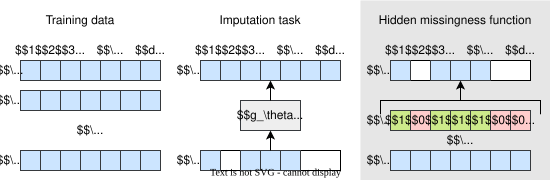
\includegraphics[width=\textwidth]{figures/versatile_imputation.pdf}}
        \caption{The problem of \textit{versatile imputation}. The training data comprises a set of complete observation-groups, $\{\myvect{y}^1, \dots,\myvect{y}^n\}$. The imputation task requires filling in the missing instances of an observation-group, $\mygroup{\myvect{y}}'$. We assume an underlying missingness mechanism that produces an incomplete observation-group, $\mygroup{\myvect{y}} \left[ \mygroup{\myvect{m}} \right]'$, by combining an unseen complete observation-group, $\mygroup{\myvect{x}}'$, and a missingness pattern, $\mygroup{\myvect{m}}'$.}
        \label{fig:versatile}
    \end{center}
    \vskip -0.4in
\end{figure}

The problem formulation that I am considering in this chapter assumes that the training data are different from the testing data. 
% we do not have access to incomplete samples from the underlying joint density between observation-groups and missingness patterns, $\myfunc{p}^{*}_{\myrv{y}, \myrv{m}}$. 
The training data consists of complete observation-groups, whereas the testing data consists of incomplete observation-groups with missingness patterns sampled from an unknown missingness density. Each observation-group has a different size, $\mycnt{d}_i$, with a specific coordinate-group, $\mygroup{\myvect{x}}^i$. I call this particular formulation \textit{versatile imputation}.
% samples from the marginal density over observation-groups, $\myfunc{p}^{*}_{\mygroup{\myrv{y}}}$.  

\crit{[In the model setup (for example, the second paragraph of 4.1.2 which begins "Formally, let {(x^i,y^i)} be the training dataset"), you might reiterate that you're treating x/Y as a bag. Say that the number of observation-instances in each observation-group need not be equal, and that the coordinates need not be the same from group to group.]}

Formally, let $\left\{ \left( \mygroup{\myvect{x}}^i, \mygroup{\myvect{y}}^i \right) \right\}_{i=1}^{\mycnt{n}}$ be the training dataset and $\left\{ \left( \mygroup{\myvect{x}}^{'i}, \mygroup{\myvect{y}} \left[ \mygroup{\myvect{m}} \right]^{'i} \right) \right\}_{i=1}^{\mycnt{n}^{'}}$ be the testing dataset. I model each observation-group in the training dataset as sampled according to the data marginal, $\mygroup{\myvect{y}}^i \overset{\mathrm{i.i.d.}}{\sim} \myfunc{p}^{*}_{\mygroup{\myrv{y}}; \, \mygroup{\myvect{x}}^i}$, where $\forall i \in \left\{ 1:\mycnt{n} \right\}$. Recall that I am treating the observation, $\mygroup{\myvect{y}}^i$, and the coordinates, $\mygroup{\myvect{x}}^i$, as an orderless bag of elements. The number of elements in each group, $\mycnt{d}_i$, need not be equal, and the coordinates, $\mygroup{\myvect{x}}$, need not be the same from group to group. 

I model each pair of observation-group and missingness pattern in the testing dataset as sampled from the underlying joint density, $\left( \mygroup{\myvect{y}}^{'i}, \mygroup{\myvect{m}}^{'i} \right) \overset{\mathrm{i.i.d.}}{\sim} \myfunc{p}^{*}_{\mygroup{\myrv{y}}, \mygroup{\myrv{m}}; \, \mygroup{\myvect{x}}^{'i}}$, where $i \in \left\{ 1:\mycnt{n}' \right\}$. For succinctness, I will omit the coordinate-group, $\mygroup{x}$, from the notation, except for where it is necessary for understanding. I show a diagram of the versatile imputation paradigm in Figure~\ref{fig:versatile}. 
% This means that the training data comprises only complete observation-groups but the testing data comprises incomplete observation-groups with an unknown missingness density. 

The goal of versatile imputation is to learn a parametric density, $\myfunc{p}^{\theta}_{\mygroup{\myrv{y}} | \mygroup{\myrv{y}} \left[ \mygroup{\myrv{m}} \right]; \mygroup{\myvect{x}}}$, called the \textit{imputation posterior}, that infers the complete observation-group, $\mygroup{\myrv{y}}$, conditional on the incomplete observation, $\mygroup{\myrv{y}} \left[ \mygroup{\myrv{m}} \right]$, and on the coordinate-group, $\mygroup{\myvect{x}}$. This density is parametrised by the trainable parameter $\theta$.

\crit{[Why this formulation? Show applicability]}

\crit{[The distinctive instance is that I allow for arbitrary missingness.]}

The challenges of versatile imputation are harder to see at first glance. From a statistical point of view, this formulation seems trivial: all we have to do is to learn the underlying joint density over the instances in the training dataset, $\myfunc{p}^{*}_{\mygroup{\myrv{y}}}$, and then generate values for the missing instances in the testing dataset in a way that maximises the probability of the testing observation-groups under the learned density, $\myfunc{p}^{\theta}_{\mygroup{\myrv{y}}}$. The imputation can be achieved with conventional statistical methods, such as the Expectation Maximisation (EM) algorithm. However, this approach is infeasible for high-dimensional data due to computational inefficiency (see Background section). Therefore, we must find an amortised method to infer the missing instances, meaning to learn to approximate the conditional density of the complete observation-group given the incomplete observation-group implied by the true data-generating process, $\myfunc{p}^{*}_{\mygroup{\myrv{y}} | \mygroup{\myrv{y}} \left[ \mygroup{\myrv{m}} \right]}$, also called the \textit{true imputation posterior}. This is where the challenge arises. 

Existing deep learning methods for versatile imputation struggle to perform imputation accurately across different \textit{missingness densities} (i.e., different settings for $\myfunc{p}^{*}_{\mygroup{\myrv{m}} | \mygroup{\myrv{y}}}$). These methods learn by first simulating missingness in the training data with an artificial missingness density, $\myfunc{p}^{\pi}_{\mygroup{\myrv{m}} | \mygroup{\myrv{y}}}$ (parametrised by $\pi$), and then training in a supervised way the imputation posterior, $\myfunc{p}^{\theta}_{\mygroup{\myrv{y}} | \mygroup{\myrv{y}} \left[ \mygroup{\myrv{m}} \right]}$, on the resulting data. Concretely, let $\left\{ \left( \mygroup{\myvect{x}}^i, \mygroup{\myvect{y}}^i, \mygroup{\myvect{m}}^i \right) \right\}_{i=1}^{\mycnt{n}}$ be the \textit{simulated training dataset}, obtained by first sampling missingness patterns according to the artificial missingness density, $\forall i \in \left\{ 1:\mycnt{n} \right\}, ~ \mygroup{\myvect{m}}^i \sim \myfunc{p}^{\pi}_{\mygroup{\myrv{m}} | \mygroup{\myrv{y}} = \mygroup{\myvect{y}}^i}$, and then applying the missingness patterns to the complete observation-groups, $\left\{ \mygroup{\myvect{y}} \left[ \mygroup{\myvect{m}} \right]^i \right\}_{i=1}^{\mycnt{n}}$. The imputation posterior is trained to maximise the log-likelihood of the simulated training dataset,
\[
    \hat{\theta} = \underset{\theta}{\mathrm{arg~max}} ~ \sum_{i=1}^{\mycnt{n}} \log \myfunc{p}^{\theta}_{\mygroup{\myrv{y}} | \mygroup{\myrv{y}} \left[ \mygroup{\myrv{m}} \right]} \left( \left. \mygroup{\myvect{y}}^i \right\vert \mygroup{\myvect{y}} \left[ \mygroup{\myvect{m}} \right]^i \right).
\]
These methods perform poorly when the artificial missingness density, $\myfunc{p}^{\pi}_{\mygroup{\myrv{m}} | \mygroup{\myrv{y}}}$, differs substantially from the true missingness density, $\myfunc{p}^{*}_{\mygroup{\myrv{m}} | \mygroup{\myrv{y}}}$ \citep{quanDeepLearningBasedImage2024}. \crit{[Show example here.]}

The formulation of versatile imputation has been neglected by the statistical literature on imputation even though it is a common problem for real-world applications. Various parallel research fields in deep learning have emerged to study special cases of this formulation, including image inpainting \citep{quanDeepLearningBasedImage2024}, image restoration \citep{suSurveyDeepLearning2022}, self-supervised pre-training \citep{heMaskedAutoencodersAre2022, devlinBERTPretrainingDeep2019,brownLanguageModelsAre2020a}, and multivariate time-series imputation \citep{kazijevsDeepImputationMissing2023}. Each of these tasks has its own set of state-of-the-art models that are fine-tuned for the characteristic missingness patterns for that task but that perform poorly on the missingness patterns characterising other tasks. For example, an image superresolution algorithm learns to impute missing pixels in a grid-like pattern but fails to impute plausibly when the missing pixels form a large continuous area \citep{chanSuperresolutionImageReconstruction2007}.

\subsection{Contribution}

In this chapter, I pull together the disparate research fields studying imputation with deep learning into a common framework. I propose a new  imputation method, the \textit{Multiple-Instance Variational Autoencoder} (MIVAE), that performs well on a variety of missingness densities. MIVAE leverages the power of the group-instance model by treating the observations, $\mygroup{\myrv{y}}$, as groups and its individual elements, $\left\{ \myrv{y}_k \right\}_{k=1}^{\mycnt{d}}$, as instances. This approach allows MIVAE not only to learn the joint density between instances $\myfunc{p}^{*}_{\mygroup{\myrv{y}}; \, \mygroup{\myvect{x}}}$, but also to approximate the true imputation conditional $\myfunc{p}^{*}_{\mygroup{\myrv{y}} | \mygroup{\myrv{y}} \left[ \mygroup{\myrv{m}} \right]}$ more closely than competing models. I evaluate the effectiveness of MIVAE on two real-world imputation tasks --- prosody control and image inpainting --- demonstrating its superior performance across various missingness densities as compared to the current state-of-the-art model, the Masked Autoencoder. 

My contributions in this chapter are threefold. Firstly, I define the problem of versatile imputation as a coherent goal of missing data imputation. Then, I propose a general approach to solve this problem and show its effectiveness empirically. Finally, I explore potential theoretical explanations for the improved performance achieved by MIVAE.

% We propose our own model for prosody generation and control, called Multiple-Instance Variational Autoencoder (MIVAE). MIVAE can be conditioned on partially specified inputs via its novel self-attention encoder, which treats the individual acoustic features as instances in an unordered set. \crit{[Why do you need a novel encoder? What is the problem with existing encoders? It deserves a paragraph about why this is hard.]}
            
\crit{[Missing big picture.]}

% Our intention is to present a novel framework for sparse control in the domain of highly-structured data. We believe that our introduction of new criteria for success (faithfulness, efficiency, and robustness) differentiates our approach from missing data imputation. For example, robust methods must produce consistent prosody across various sparsity patterns, while missing data imputation evaluates models under specific sparsity patterns (e.g., a contiguous area of the image for image inpainting). We will clarify this connection in the camera-ready paper. While we acknowledge that our work currently focuses on a single application, we assert that the identification of sparse control as a relevant and important component of human-AI interaction warrants a presentation of the general framework. We introduce an initial set of traits (faithfulness, efficiency, and robustness) applicable to the general case, not just our specific application to speech and prosody. We hope that future work can critique and build upon our analysis and evaluation, possibly adding or adjusting the traits we proposed.

% \paragraph{Background.}  We are generating speech audio. We have a TTS module converting text (in the form of phoneme embeddings) and acoustic features (in the form of a 3x matrix), plus some other labels, into audio waveform. This model is a large Transformer (called the Tacotron). The acoustic features (acoustic features) are generated by another network, called the acoustic feature Predictor (AFP). This module takes as input the text embeddings, other labels and produces the matrix of acoustic features.

% \paragraph{Problem.} The output voices are realistic, but they are not expressive or emotional. We want to be able to control the output prosody (intonation, rhythm, volume) in order to express the right emotions. The best approach to do this is to condition the AFP on some extra inputs such that the generated acoustic features.

% \paragraph{Naive approach.} The current approaches to this problem suffer from a lack of precision. Some people condition on human-provided labels like question or shouting. These are not expressive enough. There are also heuristic rules for changing

% \paragraph{Missing data problem setup.} So we have a pre-trained TTS module. We have a training set for the AFP module, consisting of tuples of (audio waveforms, text embeddings, and acoustic features). The acoustic features are extracted deterministically from the audio (they are pitch, duration and energy). We have all 3 instances per each phoneme. The task is that the AFP should take as input a matrix of (possibly missing) acoustic features, along with the text embeddings, and generate a complete matrix of acoustic features. This is called missing data imputation. The goal is that the imputation is as realistic as possible. Users provide values for the acoustic features through a set of visual sliders.

% \paragraph{Problem} Existing control methods lack precision or are cumbersome to use. On one side, there are high-level control methods using deep learning. These methods allow the user to control the synthesis either by directly modifying the values of a latent variable or providing a conditioning input, such as a label or a segmentation mask. These methods are fast and cause semantically meaningful changes to the output. However, they are imprecise and uninterpretable: you can only get so close to the desired output. On the other side, there are low-level control methods using traditional methods. These include manually editing the output, or using pre-defined heuristic rules to achieve a certain effect (e.g. change a statement into a question). They are precise, but require hours of expert human labour and are particularly difficult for high-dimensional data, like images or audio.

% \paragraph{Our solution} We propose to use the framework of MDI through the latent-group model to achieve human control that is both precise and fast, in other words, efficient. The idea is to infer the latent variable from a sparse group of acoustic features $\mygroup{X}'_i$, and then generate the complete sentence audio as output. The conditioning inputs are provided by the user by hand via a visual interface with sliders. The model is tasked with completing the missing acoustic features. We implement the model as a CVAE with an encoder network that can take as input groups of varying numbers of observation-groups instead of single observation-groups. We use two positional embeddings per instance: one sinusoidal embedding specifying the phoneme, and one learned embedding distinguishing between the 3 types of instances (pitch, energy, and duration). \crit{What is new here compared to the first description of our method. We guess we say what kind of positional embeddings and decoder we are using for the data. We also say what the variables mean.}

\section{Related Work}

\crit{[Discuss here Gaussian Processes, Neural Processes, and Transformers.]}

% \begin{figure}[t]
%     \begin{center}
%         \centerline{\includegraphics[width=0.9\columnwidth]{figures/model.pdf}}
%         \caption{Our model, MIVAE, encodes partial information and decodes a complete output. The inputs and outputs are prosodic acoustic features (acoustic features), with 3 values ($F_0$, energy and duration) for each phoneme in the sentence. \crit{\textbf{Note:} I didn't have time to update the notation, instead of $\myvect{x}$ please read $\myvect{o}$ (the partial observation-groups of the acoustic features), and instead of $k$ read $d$ (the dimensions of the data).}}
%         \label{fig:model}
%     \end{center}
%     \vskip -0.4in
% \end{figure}

\paragraph{Missing data imputation.} Missing data imputation is one of the most widely studied problems in statistics and machine learning \citep{rubinInferenceMissingData1976,campionMultipleImputationNonresponse1989,sterneMultipleImputationMissing2009}. Imputation for high-dimensional data can be divided into two main areas: 

The first area we can call \textit{dataset completion}, to which Gaussian Processes \citep{rasmussenGaussianProcessesMachine2005,jafrastehGaussianProcessesMissing2022} and matrix completion methods \citep{caiSingularValueThresholding2010} belong. These solutions address the traditional formulation of the missing data imputation problem, where, in effect, there is no training data; there is a single dataset with missingness. These methods work well for a limited dataset but cannot leverage the information contained in a large scale dataset. 

The second area we can call \textit{specific imputation}, to which image inpainting \citep{elharroussImageInpaintingReview2020}, language modelling \citep{brownLanguageModelsAre2020a}, and image superresolution \citep{chanSuperresolutionImageReconstruction2007} belong. These methods are trained on large-scale dataset for specific missingness distributions (e.g., grid-like patterns, next sentence prediction, etc.) that correspond to a real-world application.

The third area we can call \textit{representation imputation}, to which self-supervised learning methods belong \citep{heMaskedAutoencodersAre2022, tangSelfsupervisedLearningDataefficient2024}. These methods are trained on large-scale datasets, usually with random Bernoulli missingness, in order to learn robust representations of the input data, which are then used for various downstream tasks.

\paragraph{Human-in-the-loop Control.} Research on human-in-the-loop machine learning is growing rapidly~\citep{wuSurveyHumanintheloopMachine2022}. Iterative labelling improves the training of deep learning models by focusing human effort on labelling the most informative data~\citep{xinAcceleratingHumanintheloopMachine2018,chaiHumanintheloopTechniquesMachine2020}. This approach is essential for tasks like text, speech, and image generation where multiple correct answers exist for the same inputs. However, there are few works where humans control the outputs of deep models at test time. Correcting high-dimensional data manually is prohibitively costly. In the context of Computer Vision, some approaches have been studied extensively, such as inpainting~\citep{elharroussImageInpaintingReview2020} and semantic manipulation~\citep{park2019semantic}. However, even these methods struggle with generating globally consistent images~\citep{zhangCoherentImageInpainting2023}.

One approach to enable human control is to use the latent representation as input. However, not all representations are amenable for human interaction. Various methods can be applied to encourage interpretability~\citep{tschannenRecentAdvancesAutoencoderBased2018}. Structure can be imposed on the latent variables through independence assumptions~\citep{anEffectiveDirectControl2021} and hierarchical assumptions~\citep{hsuHierarchicalGenerativeModeling2019}. Self-supervised losses can also be used to disentangle concepts~\citep{sunFullyhierarchicalFinegrainedProsody2020}. Discrete latent variables are another useful method to make representations more usable for humans~\citep{vandenoordNeuralDiscreteRepresentation2017}.

Instead of striving for interpretable representations, it is also possible to focus on specific down-stream tasks. For prosody control, categorical control of representations has been successful in providing an interface for human interaction, such as for emotions~\citep{schroderEmotionalSpeechSynthesis2001} and styles~\citep{prateekOtherNewsBistyle2019}.

\paragraph{Conditioning generative models.} Generative models are a broad class of probabilistic models known for their ability to produce realistic unconditional samples for text~\citep{brownLanguageModelsAre2020a}, images~\citep{rombachHighresolutionImageSynthesis2022,rameshHierarchicalTextconditionalImage2022}, and speech~\citep{vandenoordNeuralDiscreteRepresentation2017}. Variational inference provides the tools to control (i.e.,\ condition) generative models~\citep{sohnLearningStructuredOutput2015,mirza2014conditional,winklerLearningLikelihoodsConditional2020}.

\paragraph{Inpainting.} The closest related work to our own is that on speech inpainting~\citep{borsosSpeechPainterTextconditionedSpeech2022}, itself drawing upon the vast literature on image inpainting~\citep{elharroussImageInpaintingReview2020}. However, our work explicitly addresses the problem of control. \crit{[What does this mean?]} Our introduction of new criteria for success (efficiency and robustness) differentiates us from inpainting. \crit{[Why are you introducing new criteria for success to make yourself look good?]} For example, methods in our framework must produce consistent prosody across various missingness patterns, while inpainting evaluates models under specific patterns (e.g., a contiguous area of the image). \crit{[Didn't you also choose 7 specific missingness patterns?]}

% \section{Problem formulation}

\crit{[When we do not know the group size, we write $\mycnt{d}$]}

\crit{[Set up as supervised learning problem. The covariate, x, is the coordinate. The response, y, is the observation-group. The covariate is never missing, and it's not random.]}

\crit{[Give example with images. Pixel is the instance, the image is the group. The position is x and the value is y.]}

% \crit{[Use different notation from acoustic feature and AFP.]}

% Our prosody control setup is as follows: A text-to-speech model takes as input a sentence in text form, along with corresponding acoustic features, and outputs mel-spectrograms~\citep{taylorTexttospeechSynthesis2009}. The acoustic features are generated by an acoustic feature Predictor (AFP), which takes as input the same sentence~\citep{mohanCtrlPTemporalControl2021}. The training data for the AFP comprises the following structure for each sentence: the sentence written out in phoneme-form, paired with a matrix of acoustic features containing 3 acoustic features for each phoneme in the sentence. At test time, we want to enable the user to change the values of the acoustic features by controlling the AFP through some form of conditioning. \crit{[This isn't part of the problem statement, but actually what the problem will be used for.]}

% \paragraph{Formal statement.} We are given a training dataset of pairs $\{(\myvect{x}_i, \myvect{y}_i)\}_{i=1}^N$, where $\myvect{x}_i \in \mathbb{A}^{T_i}$ is a sentence written-out in phoneme form. Let $\mathbb{A}$ be the alphabet of phonemes and $T_i$ the number of phonemes in sentence $i$. Let $\myvect{y}_i \in \mathbb{R}^{T_i \times 3}$ be a matrix of acoustic features with 3 channels for each phoneme in the sentence. We write $\myvect{y}_{i,d}$ for the acoustic features corresponding to the $d$-th element in the unrolled matrix of acoustic features, $d = T_i \times c + t$, where $c \in \{1:3\}, ~ t \in \{1:T_i\}$. \crit{[Make a figure. Why is it useful to unroll y?]}

% The actual input to the AFP will be a concatenation of the phonemes $\myvect{x}_i$ and the partial observation-group of the acoustic features $\myvect{o}_i$ with two sets of embeddings $\mathrm{emb}^T_t, \mathrm{emb}^C_c$ encoding the timepoint and the channel. \crit{[Where is $i$ in these? Also, o is not defined.]}

% At test time, the model receives complete sentences $\myvect{x}$, but incomplete observation-groups of the acoustic feature matrix $\myvect{y}$ --- some of the instances $\myvect{y}_{d}$ will be missing. We define the partial observation-group $\myvect{o}$ as a function of the full observation-group $\myvect{y}$ and a missingness pattern $\myvect{m} \in \{0, 1\}^{3 \times *}$. Let $s: (\mathbb{R}, \{0, 1\})^* \to (\mathbb{R} \cup \{\emptyset\})^*$ \crit{[Define the * notation and clarify that the input and output to the function have the same size. Also, maybe use a different notation for the empty set.]} be a function such that $\myvect{o}_i = s(\myvect{y}, \myvect{m})$, where:

% \[
%     \myvect{o}_{i,d} = s(\myvect{y}_{i,d}, \myvect{m}_{i,d}) = \left\{\begin{array}{ll} \myvect{y}_{i,d} ~ , ~ &\text{if} ~ \myvect{m}_{i,d} = 1 \\ \emptyset, &\myvect{m}_{i,d} = 0 \end{array}\right.
% \]

% \crit{[Discuss speaker labels and other non-time-dependent covariates in another section, maybe "trivial extensions" to the problem statement.]}

% \paragraph{Probabilistic model.} We assume the following probabilistic model \crit{[You need to carefully distinguish between the underlying density and the model. Otherwise your model sounds like cheating.]} to describe the testing data. \crit{[What testing data? You are writing a model for what you think the actual data will be. Call it "in-the-wild" data or something.]} Let $M \in \{0,1\}^{3 \times *}$ be a random variable selecting which dimensions of the acoustic feature random variable $Y$ are observed. Together, $M, Y$ deterministically generate the partial observation-group variable $O \in \{\emptyset, \mathbb{R}\}^{3 \times *}$ whose dimensions $O_k$ take the value $Y_k$ when $M_k = 1$, and the value $\emptyset$ when $M_k = 0$. The acoustic feature variable $Y$ and the missingness variable $M$ are independent of each other conditional on the random variable modelling the sentence $X \in \mathbb{A}^*$. Below is the factorisation of the joint density over all the variables: \crit{[Is this a random variable? Explain more.]}

% \[
%     \myfunc{p}_{X, Y, M, O} \equiv \myfunc{p}_X ~ \myfunc{p}_{Y | X} ~ \myfunc{p}_{M | X} \prod_{d=1}^* (\mathbb{1}_{O_k = Y_k, M_k = 1} + \mathbb{1}_{O_k = \emptyset, ~ M_k = 0})
% \]

% \crit{[You must define the star notation.]}

% Our ultimate goal is to learn the conditional parametric density $\myfunc{p}^\theta_{Y | X, M, O}$ that closely approximates the true unknown joint density $\mathbb{D}_{Y | X, M, O}$: \crit{[Explain more, unconventional notation. Also, the two densities must match.]}


% \[
%     \underset{\theta}{\mathrm{max}} ~ \mathbb{E}_{\myvect{x}, \myvect{y} \sim \mathbb{D}_{X,Y}, ~ \myvect{m} \sim \mathbb{D}_{M | X}} \bigl[ \log \myfunc{p}^\theta_{Y | X, O} (\myvect{y} | \myvect{x}, s(\myvect{y}, \myvect{m})) \bigr]
% \]

% Our acoustic feature predictor (AFP) is, in fact, our implementation of the conditional $\myfunc{p}^\theta_{Y | X, M, O}$. \crit{[Rewrite this sentence to clarify that we're talking about equivalence.]}

% \paragraph{Missingness density.} During training, we don't have access to samples from the true missingness density $\mathbb{D}_{M | X}$. However, we have access to $R$ samples from a family of missingness densities \crit{[What is a family? What are the densities?]} $\mathcal{M}$ to which the true density belongs $\mathbb{D}_{M | X} \in \mathcal{M}$. \crit{[Explain more.]} Let $\{\myfunc{p}^r_{M | X}\}_{r=1}^R$ be the set of sample densities from the family $\mathcal{M}$ that we have access to. \crit{[Unclear. What is this family of patterns of missingness?]} We define our evaluation metric as: \crit{[Why did you derive it in this way?]}

% \[
%     \underset{\theta}{\mathrm{max}} ~ \underset{r \in \{1:R\}}{\mathrm{min}} ~ \mathbb{E}_{\myvect{x}, \myvect{y} \sim \mathbb{D}_{X,Y}, ~ \myvect{m} \sim \myfunc{p}^r_{M | X}} \bigl[ \log \myfunc{p}^\theta_{Y | X, O} (\myvect{y} | \myvect{x}, s(\myvect{y}, \myvect{m})) \bigr]
% \]

% \crit{[Remove expectations and use pointwise for x and y. Think about the canonical form for optimising functions: Max objective over params such that constraints.]}

% The intuition behind this setup is that, if a control method performs well across a range of related missingness densities, then it is likely to generalise to an unseen density. \crit{[Clarify that this is the ultimate goal.]} The speech synthesis literature supports our assumption of related missingness densities~\citep{wagnerExperimentalTheoreticalAdvances2010}; human users choose to control prosody in a few distinct but closely related ways. \crit{[So is it not that hard? Why do you need a general method?]}

\section{Conventional approach: Masked autoencoders}
\label{sec:conventional-approach}

\begin{figure}[t]
    \begin{center}
        \centerline{\includegraphics[width=\columnwidth]{figures/encoder_last.pdf}}
        \caption{The self-attention encoder. The control points of the partial input are treated as an unordered bag of instances. They are aggregated into a fixed-length vector by a self-attention mechanism. \crit{[Change the figure with the new notation.]}}
        \label{fig:encoder}
    \end{center}
    \vskip -0.4in
\end{figure}

In this section, I describe the conventional approach for versatile imputation: Masked Autoencoders (MAE) \citep{vincentExtractingComposingRobust2008,bengioGeneralizedDenoisingAutoencoders2013,heMaskedAutoencodersAre2022}. I use this method both as a baseline for evaluation and a starting point for developing my own approach. I chose the masked autoencoder as a baseline because it is both flexible and conceptually simple. It is frequently employed for a wide range of machine learning tasks, including image synthesis \citep{heMaskedAutoencodersAre2022}, language modelling \citep{devlinBERTPretrainingDeep2019}, and tabular data imputation \citep{gondaraMIDAMultipleImputation2018}. Masked autoencoders are the state-of-the-art in self-supervised learning for images and text \citep{tangSelfsupervisedLearningDataefficient2024}. They are also the starting point for the method I propose in this chapter, which allows me to study the marginal improvement brought by each original component introduced by my model (see Section~\ref{sec:mivae-evaluation}).

The masked autoencoder is a variational autoencoder \citep{kingma2013auto,rezende2014stochastic} trained to impute missing instances by encoding incomplete observation-groups, $\mygroup{\myrv{y}} \left[ \mygroup{\myrv{m}} \right]$, and decoding complete observation-groups, $\tilde{\mygroup{\myrv{y}}}$, which are then measured against the ground-truth complete observation-groups, $\mygroup{\myrv{y}}$. The incomplete observation-groups are created by synthesising a pattern of missingness, $\mygroup{\myrv{m}}$, according to a chosen missingness density (e.g., $\mathrm{Ber} \left( \pi = 0.5 \right)$), and then applying the pattern to the ground-truth observation-group, resulting in $\mygroup{\myrv{y} \left[\myrv{m}\right]}$. The autoencoder is then deployed at test-time by encoding incomplete observation-groups and decoding complete observation-groups. Typically, the main challenge with the masked autoencoder is how to design an encoder architecture that can take incomplete observation-groups as input. I will discuss the different options in this section.

Formally, the masked autoencoder comprises a generative density, $\myfunc{p}^{\theta}_{\mygroup{\myrv{y}} | \myrv{w}}$, parametrised by $\theta$ (the \textit{decoder}), and a variational latent posterior density, $\myfunc{q}^{\phi}_{\myrv{w} | \mygroup{\myrv{y}}}$, parametrised by $\phi$ (the \textit{encoder}). Like the variational autoencoder, the model is trained to maximise a lower bound (ELBO) to the log-likelihood of the data. Unlike the variational autoencoder, the encoder takes as input incomplete observation-groups. The ELBO for a single training observation-group, $\mygroup{\myvect{x}}^i$, and pattern of missingness, $\mygroup{\myvect{m}}^i$, for $i \in \left\{1:\mycnt{n}\right\}$, has the form: \crit{[Show full derivation.]}
\begin{equation} \label{eq:masked-elbo}
\begin{split}
    \log \myfunc{p}^{\theta}_{\mygroup{\myrv{y}}} \left( \mygroup{\myvect{y}}^i \right)
    \, &= \, 
    \int_{\myvect{w}} \myfunc{q}^{\phi}_{\myrv{w} | \mygroup{\myrv{y}}} \left( \myvect{w} \left\vert \mygroup{\myvect{y}} \left[ \mygroup{\myvect{m}} \right]^i \right. \right) \left[ \log \myfunc{p}^{\theta}_{\mygroup{\myrv{y}}} \left( \mygroup{\myvect{y}}^i \right) \right] \, d \myvect{w} \\
    \, &= \, 
    \int_{\myvect{w}} 
    \myfunc{q}^{\phi}_{\myrv{w} | \mygroup{\myrv{y}}} \left( \myvect{w} \left\vert \mygroup{\myvect{y}} \left[ \mygroup{\myvect{m}} \right]^i \right. \right) 
    \left[ \log \frac{\myfunc{p}^{\theta}_{\mygroup{\myrv{y}} | \myrv{w}} \left( \left. \mygroup{\myvect{y}}^i \right\vert \myvect{w} \right) ~ \myfunc{p}^{\theta}_{\myrv{w}} \left( \myvect{w}\right)}{\myfunc{p}^{\theta}_{\myrv{w} | \mygroup{\myrv{y}}} \left( \myvect{w} \left\vert \mygroup{\myvect{y}}^i \right. \right)}\right] \, d \myvect{w} \\
    &= \, 
    \int_{\myvect{w}} \myfunc{q}^{\phi}_{\myrv{w} | \mygroup{\myrv{y}}} \left( \myvect{w} \left\vert \mygroup{\myvect{y}} \left[ \mygroup{\myvect{m}} \right]^i \right. \right) 
    \left[ \log \myfunc{p}^{\theta}_{\mygroup{\myrv{y}} | \myrv{w}} 
    - \log \frac{\myfunc{q}^{\phi}_{\myrv{w} | \mygroup{\myrv{y}}} \left( \myvect{w} \left\vert \mygroup{\myvect{y}} \left[ \mygroup{\myvect{m}} \right]^i \right. \right)}{\myfunc{p}^{\theta}_{\myrv{w}} \left( \myvect{w} \right)} 
    + \log \frac{\myfunc{q}^{\phi}_{\myrv{w} | \mygroup{\myrv{y}}} \left( \myvect{w} \left\vert \mygroup{\myvect{y}} \left[ \mygroup{\myvect{m}} \right]^i \right. \right)}{\myfunc{p}^{\theta}_{\myrv{w} | \mygroup{\myrv{y}}} \left( \myvect{w} \left\vert \mygroup{\myvect{y}}^i \right. \right)} \right] \, d\myvect{w} \\
    \, &\geq \, 
    \underbrace{\mathbb{E}_{\myvect{w} \sim \myfunc{q}^{\phi}_{\myrv{w} | \mygroup{\myrv{y}} = \mygroup{\myvect{y}} \left[ \mygroup{\myvect{m}} \right]^i }} 
    \left[ \log \myfunc{p}^{\theta}_{\mygroup{\myrv{y}} | \myrv{w}} \left( \left. \mygroup{\myvect{y}}^i \right\vert \myvect{w} \right) \right] }_{\text{Reconstruction loss}}
    \, - \,
    \kl[\bigg]{\myfunc{q}^{\phi}_{\myrv{w} | \mygroup{\myrv{y}} = \mygroup{\myvect{y}} \left[ \mygroup{\myvect{m}} \right]^i}}{\myfunc{p}_{\myrv{w}}},
\end{split}
\end{equation}
where the pattern of missingness, $\mygroup{\myvect{m}}^i$, is sampled from a chosen missingness density. The most common choice is to sample each instance of the missingness pattern, $\myvect{m}^i_k, ~ \forall k \in \{1:\mycnt{d}_i\}$, independently from a Bernoulli density with parameter 0.5. This way, each pattern of missingness has an equal probability of occurring. The imputation posterior, $\myfunc{p}^{\theta}_{\mygroup{\myrv{y}} | \mygroup{\myrv{y}} \left[ \mygroup{\myrv{m}} \right]}$, is computed by first sampling the latent variable from the variational posterior, $\myfunc{q}^{\phi}_{\myrv{w} | \mygroup{\myrv{y}}}$, and then using the latent variable to condition the generative posterior, $\myfunc{p}^{\theta}_{\mygroup{\myrv{y}} | \myrv{w}}$:
\[
    \myfunc{p}^{\theta}_{\mygroup{\myrv{y}} | \mygroup{\myrv{y}} \left[ \mygroup{\myrv{m}} \right]} \left( \mygroup{\myvect{y}} \left\vert \mygroup{\myvect{y}} \left[ \mygroup{\myvect{m}} \right] \right. \right)
    = 
    \int_{\myvect{w} \in \mathbb{R}^{\mydim{w}}} \myfunc{p}^{\theta}_{\mygroup{\myrv{y}} | \myrv{w}} \left( \left. \mygroup{\myvect{y}} \right\vert \myvect{w} \right) 
    ~
    \myfunc{q}^{\phi}_{\myrv{w} | \mygroup{\myrv{y}}} \left( \myvect{w} \left\vert \mygroup{\myvect{y}} \left[ \mygroup{\myvect{m}} \right] \right. \right) \, d\myvect{w}.
\]  

\paragraph{Encoder architecture.} The question is how to implement an encoder that can take as input observation-groups of varying size and possibly missing instances. There are many options for solving to this problem, but the architecture on which I will be focusing in this chapter is \textit{self-attention} \citep{vaswaniAttentionAllYou2017}. This architecture involves passing the instances of the observation-group, $\mygroup{\myrv{y}}$, as an orderless bag of inputs to a system of networks whose computation is agnostic with respect to the order of its inputs. To each instance in the observation-group, a fixed-length vector, called a \textit{positional embedding}, is concatenated in order to allow the networks ascertain the relative positions of the instances. The specific encoder architecture we will be considering is the one introduced by \citet{ilseAttentionbasedDeepMultiple2018} illustrated in Figure~\ref{fig:encoder}. I will be using the same encoder architecture for both the conventional model (masked autoencoders) and my proposed method.

Their encoding process starts with each instance of the observation-group, $\myvect{y}_k \in \mathbb{R}^{\mydim{y}}$, where $k \in \left\{1:\mycnt{d}\right\}$ indexes the instances within a group. The positional embeddings, $\myvect{x}_k \in \mathbb{R}^{\mydim{x}}$, are concatenated with $\myvect{y}_k$, to produce an extended instance vector $[ \myvect{y}_k, \myvect{x}_k ]$. By default, the positional embeddings follow a sinusoidal pattern \citep{vaswaniAttentionAllYou2017}. A set of hidden representations, $\myvect{h}_k \in \mathbb{R}^{\mydim{h}}$, are computed as $\myvect{h}_k = \mathrm{ReLU} \left( \mathbf{E} \cdot \left[ \myvect{y}_k, \myvect{e}_k \right]^T \right)$, where $\mathbf{E} \in \mathbb{R}^{\mydim{h} \times (\mydim{y} + \mydim{x})}$ is a matrix of trainable weights. Each intermediate representation, $\myvect{h}_k$, is then transformed into a value vector, $\myvect{v}_k \in \mathbb{R}^{\mydim{z}}$, via a perceptron, $\myvect{v}_k = \tanh \left( \mathbf{V} \cdot \myvect{h}_k^T \right)$, where $\mathbf{V} \in \mathbb{R}^{\mydim{z} \times \mydim{h}}$. A set of key-query products, $\myvect{b}_k \in \mathbb{R}$, are computed as folows, $\myvect{b}_k = \myvect{w}^T \left( \tanh \left( \mathbf{Q} \myvect{h}_k^T \right) \odot \mathrm{sigm} \left( \mathbf{K} \myvect{h}_k^T \right) \right)$, where $\myvect{w} \in \mathbb{R}^{\mydim{z}}$, $\mathbf{Q} \in \mathbb{R}^{\mydim{z} \times \mydim{h}}$, and $\mathbf{K} \in \mathbb{R}^{\mydim{z} \times \mydim{h}}$ are trainable weights. A set of attention weights, $\myvect{a}_k \in [0, 1]$, are computed as follows, $\myvect{a}_k = \exp \left( \myvect{b}_k \right) / \sum_{l=1}^{K} \exp \left( \myvect{b}_l \right)$. The attention weights are used to compute a weighted sum of value vectors, yielding a group-level embedding, $\myvect{w} \in \mathbb{R}^{\mydim{z}}$, computed as follows, $\myvect{w} = \sum_{k=1}^{\mycnt{d}} \myvect{a}_k \myvect{v}_k$.

% \paragraph{Limitation.} Training the variational autoencoder with incomplete data raises the risk that the generative model \textit{might not} learn to match the training data. As reviewed in the Background section, in order for the evidence lower-bound to become equal to the data log-likelihood (Equation~\ref{eq:masked-elbo}) the variational latent density, $\myfunc{q}^{\phi}_{\myrv{w} | \mygroup{\myrv{y}}}$, must match the latent posterior implied by the true data-generating process, $\myfunc{p}^{*}_{\myrv{w} | \mygroup{\myrv{y}}}$. If they match, then the training process will maximise the likelihood of the generative model, $\myfunc{p}^{\theta}_{\mygroup{\myrv{y}} | \myrv{w}}$, with respect to the training data (under some assumptions). If, however, we feed incomplete observation-groups to the variational latent posterior, $\myfunc{q}^{\phi}_{\myrv{w} | \mygroup{\myrv{y}} = \mygroup{\myvect{y}} \left[ \mygroup{\myvect{m}} \right]}$, during training, then variational density cannot match the true latent posterior conditioned on complete observation-groups, $\myfunc{p}^{*}_{\myrv{w} | \mygroup{\myrv{y}} = \mygroup{\myvect{y}}}$, because it lacks the information contained in the missing instances of the observation-groups. This may impact whether the generative model, $\myfunc{p}^{\theta}_{\mygroup{\myrv{y}} | \myrv{w}}$, learns to match the training data. The model I propose in this chapter will address this limitation.


\section{My approach: Multiple-instance VAE}

\begin{figure}[t]
    \begin{center}
        \centerline{\includegraphics[width=0.6\columnwidth]{figures/new_prob.pdf}}
        \caption{Our probabilistic graphical model for the versatile imputation problem. Instance $k$ of the partial observation-group-group, $\myrv{y} \left[ \myrv{m} \right]_k$, is generated by applying an instance of the missingness pattern, $\myrv{m}_k$, to an instance of the complete observation-group-group, $\myrv{y}_k$, with the missingness pattern. During training, only the complete observation-group-group, $\mygroup{\myrv{y}}$, and the corresponding coordinates, $\mygroup{\myvect{x}}$, are observed. During testing, only the partial observation-group-group, $\mygroup{\myrv{y}} \left[ \mygroup{\myrv{m}} \right]$, the coordinates, $\mygroup{\myvect{x}}$, and the missingness pattern, $\mygroup{\myrv{m}}$, are observed.}
        \label{fig:mivae-pgm}
    \end{center}
    \vskip -0.4in
\end{figure}

I propose a parametric model and training procedure, the Multiple-Instance Variational Autoencoder (MIVAE), that can perform versatile imputation across different missingness densities. MIVAE follows the paradigm of the Variational Autoencoder \citep{sohnLearningStructuredOutput2015} applied to grouped data. In the case of versatile imputation, the group consists of the set of $\mycnt{d}$ instances, $\mygroup{\myrv{y}} = \left\{ \myrv{y}_1, \dots, \myrv{y}_{\mycnt{d}} \right\}$.

\paragraph{Training objective.} The main innovation underpinning the MIVAE is a training objective that enables the model to learn to impute incomplete observation-groups without being trained explicitly with incomplete observation-groups. The training objective of my model starts from the conventional loss function of the variational autoencoder, the Evidence-Lower Bound (ELBO) \citep{kingma2013auto,rezende2014stochastic}, applied with one fixed-dimensional latent variable, $\myrv{w}$, per observation-group variable, $\mygroup{\myrv{y}}$.
My formulation of the ELBO for the $i$-th training observation-group, $\myvect{y}^i$, has the form of the ELBO of the original variational autoencoder (see Background section), only applied at the group level: \crit{[Show full derivation.]}
\begin{equation} \label{eq:MIVAE-elbo}
\begin{split} 
    \log \myfunc{p}^{\theta}_{\mygroup{\myrv{y}}} \left( \mygroup{\myvect{y}}^i \right)
    \, &= \, 
    \int_{\myvect{w}} \myfunc{q}^{\phi}_{\myrv{w} | \mygroup{\myrv{y}}} \left( \myvect{w} \left\vert \mygroup{\myvect{y}}^i \right. \right) \left[ \log \myfunc{p}^{\theta}_{\mygroup{\myrv{y}}} \left( \mygroup{\myvect{y}}^i \right) \right] \, d \myvect{w} \\
    \, &= \, 
    \int_{\myvect{w}} 
    \myfunc{q}^{\phi}_{\myrv{w} | \mygroup{\myrv{y}}} \left( \myvect{w} \left\vert \mygroup{\myvect{y}}^i \right. \right) 
    \left[ \log \frac{\myfunc{p}^{\theta}_{\mygroup{\myrv{y}} | \myrv{w}} \left( \left. \mygroup{\myvect{y}}^i \right\vert \myvect{w} \right) ~ \myfunc{p}^{\theta}_{\myrv{w}} \left( \myvect{w}\right)}{\myfunc{p}^{\theta}_{\myrv{w} | \mygroup{\myrv{y}}} \left( \myvect{w} \left\vert \mygroup{\myvect{y}}^i \right. \right)}\right] \, d \myvect{w} \\
    \, &= \, 
    \int_{\myvect{w}} \myfunc{q}^{\phi}_{\myrv{w} | \mygroup{\myrv{y}}} \left( \myvect{w} \left\vert \mygroup{\myvect{y}}^i \right. \right) 
    \left[ \log \myfunc{p}^{\theta}_{\mygroup{\myrv{y}} | \myrv{w}} 
    - \log \frac{\myfunc{q}^{\phi}_{\myrv{w} | \mygroup{\myrv{y}}} \left( \myvect{w} \left\vert \mygroup{\myvect{y}}^i \right. \right)}{\myfunc{p}^{\theta}_{\myrv{w}} \left( \myvect{w} \right)} 
    + \log \frac{\myfunc{q}^{\phi}_{\myrv{w} | \mygroup{\myrv{y}}} \left( \myvect{w} \left\vert \mygroup{\myvect{y}}^i \right. \right)}{\myfunc{p}^{\theta}_{\myrv{w} | \mygroup{\myrv{y}}} \left( \myvect{w} \left\vert \mygroup{\myvect{y}}^i \right. \right)} \right] \, d\myvect{w} \\ 
    & \, \geq \, 
    \underbrace{\mathbb{E}_{\myvect{w} \sim \myfunc{q}^{\phi}_{\myrv{w} | \mygroup{\myrv{y}} = \mygroup{\myvect{y}}^i }} 
    \left[ \log \myfunc{p}^{\theta}_{\mygroup{\myrv{y}} | \myrv{w}} \left( \left. \mygroup{\myvect{y}}^i \right\vert \myvect{w} \right) \right]
    - 
    \kl[\bigg]{\myfunc{q}^{\phi}_{\myrv{w} | \mygroup{\myrv{y}} = \mygroup{\myvect{y}}^i}}{\myfunc{p}_{\myrv{w}}}}_{\text{Standard ELBO}}
\end{split}
\end{equation}

The advantage of the traditional ELBO objective (Equation~\ref{eq:MIVAE-elbo}) over the MAE ELBO objective (Equation~\ref{eq:masked-elbo}) is that it trains the generative model, $\myfunc{p}^{\theta}_{\mygroup{\myrv{y}} | \myrv{w}}$, with maximum likelihood estimation (given a sufficiently expressive encoder). Recall from the Background section that if the variational latent posterior density, $\myfunc{q}^{\phi}_{\myrv{w} | \mygroup{\myrv{y}}}$, becomes equivalent to the latent posterior implied by the generative model, $\myfunc{p}^{\theta}_{\myrv{w} | \mygroup{\myrv{y}}}$, then the ELBO for observation-group $i$ becomes equal to the log-likelihood of the generative model with respect to the data, $\log \myfunc{p}^{\theta}_{\mygroup{\myrv{y}}} \left( \mygroup{\myvect{y}}^i \right)$. Given a sufficiently expressive encoder, $\myfunc{q}^{\phi}_{\myrv{w} | \mygroup{\myrv{y}}}$, the traditional ELBO can satisfy this requirement. However, the variational latent posterior of the MAE is conditioned on incomplete observations, $\mygroup{\myvect{y}} \left[ \mygroup{\myvect{m}} \right]^i$, so it does not have access to the information in the missing components of the observation-group, $\mygroup{\myvect{y}}^i$. Therefore, the variational latent posterior, $\myfunc{q}^{\phi}_{\myrv{w} | \mygroup{\myrv{y}} = \mygroup{\myvect{y}} \left[ \mygroup{\myvect{m}} \right]^i}$, cannot be equivalent to the generative latent posterior, $\myfunc{p}^{\theta}_{\myrv{w} | \mygroup{\myrv{y}} = \mygroup{\myvect{y}}^i}$, except for degenerate cases where the same information is present in the incomplete observation-group regardless of the missingness pattern (e.g. an example would be a dataset of images where the left half of an image is always identical to the right half of that image, and there are only two possible patterns of missingness: left-half missing or right-half missing).

\subsection{Alignment loss} 

In addition to the ELBO, I propose an auxiliary loss function, which I call the ``alignment'' loss. On its own, the ELBO objective is insufficient for training an inference model that correctly aligns two incomplete views of the same underlying complete observation in the representation space~\citep{heMaskedAutoencodersAre2022,zhangHowMaskMatters2022}. This means that, for a given observation-group, $\mygroup{\myvect{y}}$, two different missingness patterns, $\mygroup{\myvect{m}}^1$ and $\mygroup{\myvect{m}}^2$, will produce two incomplete observations, $\mygroup{\myvect{y}} \left[ \mygroup{\myvect{m}}^1 \right]$ and $\mygroup{\myvect{y}} \left[ \mygroup{\myvect{m}}^2 \right]$, that are mapped by the encoder to two different distributions over the latent space, $\myfunc{q}^{\phi}_{\myrv{w} | \mygroup{\myrv{y}} = \mygroup{\myvect{y}} \left[ \mygroup{\myvect{m}}^1 \right]}$ and $\myfunc{q}^{\phi}_{\myrv{w} | \mygroup{\myrv{y}} = \mygroup{\myvect{y}} \left[ \mygroup{\myvect{m}}^2 \right]}$. Ideally, we would like these two densities to overlap as much as possible with eachother, and as little as possible with variational posterior densities conditioned on other observation-groups, such as $\myfunc{q}^{\phi}_{\myrv{w} | \mygroup{\myrv{y}} = \mygroup{\myvect{y}}'}$, where $\mygroup{\myvect{y}} \neq \mygroup{\myvect{y}}'$. However, \citet{zhangHowMaskMatters2022} have discovered empirically that training a variational autoencoder with the MAE ELBO (Equation~\ref{eq:masked-elbo}) improves the representational alignment over the model trained with the traditional ELBO (Equation~\ref{eq:MIVAE-elbo}), thereby showing that there is space for improving the alignment for the traditional ELBO.

In order to encourage the representational alignment between incomplete views of the same complete observation, I propose the auxiliary alignment loss. This loss pushes the variational latent posterior conditioned on one observation-group, $\mygroup{\myvect{y}}$, to be closer to a combination of $\mycnt{d}$ variational latent posteriors, each conditioned on a different instance of the observation, $\myvect{y}_k$. The alignment loss has the form:
\begin{equation} \label{eq:MIVAE-imputation-loss}
    \mathrm{ALGN} \left( \phi, \mygroup{\myvect{y}}^i, \mygroup{\myvect{x}}^i \right) = \kl[\Bigg]{ 
    \underbrace{\myfunc{q}^{\phi}_{\myrv{w} | \mygroup{\myrv{y}} = \mygroup{\myvect{y}}^i}}_{\text{Posterior given one group}} 
    }{ 
    \myfunc{h} \left( \myrv{w}, \mygroup{\myvect{y}}^i \right) \, \prod_{k=1}^{\mycnt{d}_i} \underbrace{\myfunc{q}^{\phi}_{\myrv{w} | \mygroup{\myrv{y}} = \left[ \myvect{y}^i_k \right]; \, \myvect{x}^i_k}}_{\text{Posterior given one instance}} }
\end{equation}
where $\myfunc{q}^{\phi}_{\myrv{w} | \mygroup{\myrv{y}} = \left[ \myvect{y}^i_k \right]; \, \myvect{x}^i_k}$ is the variational latent posterior density conditioned on the $k$-th instance of the observation-group, $\myvect{y}^i_k$. This is calculated by feeding to the encoder a single instance, $\myvect{y}^i_k$, as if it were a complete observation-group. The function $\myfunc{h}\left( \myvect{w}, \mygroup{\myvect{y}}^i \right)$ has the form:
\begin{equation} \label{eq:MIVAE-h-func}
    \myfunc{h}\left( \myvect{w}, \mygroup{\myvect{y}}^i \right) = \frac{\prod_{k=1}^{\mycnt{d}_i} \myfunc{p}^{*}_{\myrv{y}_k} \left( \myvect{y}^i_k \right)}{\myfunc{p}^{*}_{\mygroup{\myrv{y}}} \left( \mygroup{\myvect{y}}^i \right)} ~ \frac{1}{\left( \myfunc{q}_{\myrv{w}} (\myvect{w}) \right)^{\mycnt{d}_i - 1}},
\end{equation}
where the density $\myfunc{q}_{\myrv{w}} (\myvect{w})$ is implied by the true density of observation-groups, $\myfunc{p}^{*}_{\mygroup{\myrv{y}}} (\myvect{x})$, and the variational latent posterior, $\myfunc{q}^{\phi}_{\myrv{w} | \mygroup{\myrv{y}}} \left( \myvect{w} | \mygroup{\myvect{y}} \right)$:
\begin{equation}
    \myfunc{q}^{\phi}_{\myrv{w}} (\myvect{w}) = \int\limits_{\myvect{y} \in \mathbb{R}^{*}} \myfunc{q}^{\phi}_{\myrv{w} \left\vert \mygroup{\myrv{y}} \right. } \left( \myvect{w} \left\vert \mygroup{\myvect{y}} \right. \right) \, \myfunc{p}^{*}_{\mygroup{\myrv{y}}} \left( \mygroup{\myvect{y}} \right) \, d\myvect{y}.
\end{equation}

The overall loss function of the MIVAE for the training group $i$ is a combination between the traditional ELBO (Equation~\ref{eq:MIVAE-elbo}) and the alignment loss (Equation~\ref{eq:MIVAE-imputation-loss}):
\begin{equation}
    \lambda ~ \mathrm{ALGN} \left( \phi, \mygroup{\myvect{y}}^i, \mygroup{\myvect{x}}^i \right) - \mathrm{ELBO} \left( \theta, \phi, \mygroup{\myvect{y}}^i, \mygroup{\myvect{x}}^i \right),
\end{equation}
where $\lambda$ is a hyperparameter controlling the strength of the alignment loss. In my experiments, I set $\lambda = 10^3$.

\paragraph{Interpretation.} The alignment loss (Equation~\ref{eq:MIVAE-imputation-loss}) is the KL-divergence between the variational latent posterior density, $\myfunc{q}^{\phi}_{\myrv{w} | \mygroup{\myrv{y}} = \left[ \myvect{y}^i_k \right] ; \, \myvect{x}^i_k}$, and a function of the product of variational latent posteriors conditioned on each individual instance, $\myfunc{h} \left( \myrv{w}, \myvect{y}^i \right) ~ \prod_{k=1}^{\mycnt{d}_i} \myfunc{q}^{\phi}_{\myrv{w} | \mygroup{\myrv{y}} = \left[ \myvect{y}^i_k \right] ; \, \myvect{x}^i_k}$. The alignment loss has two important properties: 
\begin{enumerate}
    \item The value of the alignment loss is always greater than or equal to 0 because it is a KL-divergence. Therefore, subtracting its value from the ELBO preserves the inequality, so the overall loss still maximises a lower bound to the data log-likelihood, $\log \myfunc{p}^{\theta}_{\mygroup{\myrv{y}}} \left( \mygroup{\myvect{y}}^i \right)$.
    \item The value of the alignment loss becomes equal to 0 if the variational latent posterior conditioned on instance $k$ of the observation-group, $\myfunc{q}^{\phi}_{\myrv{w} | \mygroup{\myrv{y}} = \left[ \myvect{y}^i_k \right]; \, \mygroup{x}^i}$, is equal to the \textit{implied} variational latent posterior conditioned on the same instance $k$, $\myfunc{q}^{\phi}_{\myrv{w} | \myrv{y}_k = \myvect{y}^i_k; \, \mygroup{\myvect{x}}^i}$. The implied posterior cannot be computed directly but it is equivalent to the marginal contribution brought by instance $\myvect{y}^i_k$ to the variational latent posterior conditioned on a full observation-group, $\mygroup{\myvect{y}}^i$:
    \begin{equation} \label{eq:MIVAE-implied}
        \forall \myvect{w} \in \mathbb{R}^{\mydim{z}}, ~ \forall \mycnt{d} \in \mathbb{N}, ~ \forall \myvect{x} \in \mathbb{R}^{\mycnt{d}}, \quad \myfunc{q}^{\phi}_{\myrv{w} | \myrv{y}_k} \left( \myvect{w} \left\vert \myvect{y}_k \right. \right) = \int_{\myvect{y}_{-k}} \myfunc{q}^{\phi}_{\myrv{w} | \mygroup{\myrv{y}}} \left( \myvect{w} \left\vert \mygroup{\myvect{y}} \right. \right) \, \myfunc{q}^{\phi}_{\myrv{y}_{-k} | \myrv{y}_k} \left( \myvect{y}_{-k} | \myvect{y}_k \right) \, d\myvect{y}_{-k},
    \end{equation}
    where $\myvect{y}_{-k}$ denotes all the instances of $\mygroup{\myvect{y}}$ except for instance $k$ (i.e., $\myvect{y}_{-k} = \myvect{x}_{\{1:\mycnt{d}\} \setminus \{k\}}$).

    \paragraph{Lemma.} Formally, $\forall i \in \{1 : \mycnt{n}\}$, 
    \[
        \forall k \in \{1 : \mycnt{d}_i\}, 
        ~ \myfunc{q}^{\phi}_{\myrv{w} | \mygroup{\myrv{y}} = \left[ \myvect{y}^i_k \right]; \, \myvect{x}^i_k} \equiv \myfunc{q}^{\phi}_{\myrv{w} | \myrv{y}_k = \myvect{y}^i_k; \, \mygroup{\myvect{x}}^i}
        \implies 
        \underbrace{
            \kl[\Bigg]{ \myfunc{q}^{\phi}_{\myrv{w} | \mygroup{\myrv{y}} = \mygroup{\myvect{y}}^i} }{ \myfunc{h} \left( \myrv{w}, \mygroup{\myvect{y}}^i \right) \, \prod_{k=1}^{\mycnt{d}_i} \myfunc{q}^{\phi}_{\myrv{w} | \mygroup{\myrv{y}} = \left[ \myvect{y}^i_k \right]; \, \myvect{x}^i_k }}
        }_{\text{Alignment loss}} = 0.
    \]

    \paragraph{Proof sketch.} \crit{[The proof is in the appendix.]} This result becomes obvious once we decompose the variational latent posterior conditioned on the complete observation-group, $\myfunc{q}^{\phi}_{\myrv{w} | \mygroup{\myrv{y}} = \mygroup{\myvect{y}}^i}$, in terms of a product of implied variational latent posteriors conditioned on each instance of the observation-group, $\myfunc{q}^{\phi}_{\myrv{w} | \myrv{y}_k = \myvect{y}^i_k}$:
    \[
        \myfunc{q}^{\phi}_{\myrv{w} | \mygroup{\myrv{y}} = \mygroup{\myvect{y}}^i} \equiv \myfunc{h} \left( \myrv{w}, \mygroup{\myvect{y}}^i \right) \, \prod_{k=1}^{\mycnt{d}_i} \myfunc{q}^{\phi}_{\myrv{w} | \myrv{y}_k = \myvect{y}^i_k; \, \mygroup{\myvect{x}}^i }.
    \]
    This decomposition is identical to the term on the left-hand side of the KL-divergence in Equation~\ref{eq:MIVAE-imputation-loss}, except for the difference between the posterior, $\myfunc{q}^{\phi}_{\myrv{w} | \mygroup{\myrv{y}} = \left[ \myvect{y}^i_k \right]; \, \myvect{x}^i_k}$, and the implied posterior, $\myfunc{q}^{\phi}_{\myrv{w} | \myrv{y}_k = \myvect{y}^i_k; \, \mygroup{\myvect{x}}^i}$.
\end{enumerate}

The difference between the posterior, $\myfunc{q}^{\phi}_{\myrv{w} | \mygroup{\myrv{y}} = \left[ \myvect{y}^i_k \right]; \, \myvect{x}^i_k}$, and the implied posterior, $\myfunc{q}^{\phi}_{\myrv{w} | \myrv{y}_k = \myvect{y}^i_k; \, \mygroup{\myvect{x}}^i }$, is crucial to the efficacy of the alignment loss. The implied posterior, $\myfunc{q}^{\phi}_{\myrv{w} | \myrv{y}_k = \myvect{y}^i_k; \, \mygroup{\myvect{x}}^i}$, is the gold-standard for imputation. It reflects the maximum information that can be extracted from one observation-group variable instance, $\myrv{y}_k$, to predict the output of the encoder, $\myfunc{q}^{\phi}_{\myrv{w} | \mygroup{\myrv{y}}}$. However, it is very expensive to compute, as it requires integration (see Equation~\ref{eq:MIVAE-implied}). The actual posterior, $\myfunc{q}^{\phi}_{\myrv{w} | \mygroup{\myrv{y}} = \left[ \myvect{y}^i_k \right]; \, \myvect{x}^i_k}$, is easy to compute, but it only reflects the information that the encoder actually extracts from one observation-group variable instance, $\myrv{y}_k$. 

The alignment loss is a method for maximising the information extraction of the encoder without having to train with any missing data. As the KL-divergence between the two is minimised, the actual posterior, $\myfunc{q}^{\phi}_{\myrv{w} | \mygroup{\myrv{y}} = \left[ \myvect{y}^i_k \right]; \, \myvect{x}^i_k}$, is pushed to extract more information from the input than it would extract under normal ELBO training. The advantage of this method is its data efficiency: every instance of every training observation-group receives a training signal every epoch as if it were the only non-missing instance in the observation-group.

Another advantage of the alignment loss is that, if it reaches the value 0 (and if the variational latent poserior, $\myfunc{q}^{\phi}_{\myrv{w} | \mygroup{\myrv{y}}}$, becomes equivalent to the generative latent posterior, $\myfunc{p}^{\theta}_{\myrv{w} | \mygroup{\myrv{y}}}$), then the generative model $\myfunc{p}^{\theta}_{\mygroup{\myrv{y}} | \myrv{w}}$ is trained with maximum likelihood estimation. By contrast, the method of training with missing values never maximises the data log-likelihood directly because the variational latent posterior conditioned on incomplete observation-groups, $\myfunc{q}^{\phi}_{\myrv{w} | \mygroup{\myrv{y}} = \mygroup{\myvect{y}} \left[ \mygroup{\myvect{m}} \right]}$, will never be exactly equivalent to the generative latent posterior conditioned on complete observation-groups, $\myfunc{p}^{*}_{\myrv{w} | \mygroup{\myrv{y}} = \mygroup{\myvect{y}}}$, because it lacks the information from the missing instances. 

\paragraph{Implementation.} The main challenge involved in implementing the alignment loss is how to compute the function $\myfunc{h} \left( \myvect{w}, \mygroup{\myvect{y}} \right)$ (see Equation~\ref{eq:MIVAE-h-func}) in a differentiable way. The issue is that the expression of $h$ involves two implicit densities: the density of the observation-groups implied by the true data-generating process, $\myfunc{p}^{*}_{\mygroup{\myrv{y}}}$, and the marginal variational density of the latent variable, $\myfunc{q}_{\myrv{w}}$: 
\[
    \myfunc{h} \left( \myvect{w}, \mygroup{\myvect{y}} \right) = \underbrace{\frac{\prod_{k=1}^{\mycnt{d}_i} \myfunc{p}^{*}_{\myrv{y}_k} \left( \myvect{y}^i_k \right)}{\myfunc{p}^{*}_{\mygroup{\myrv{y}}} \left( \mygroup{\myvect{y}}^i \right)}}_{\text{true densities}} ~ \underbrace{\frac{1}{\left( \myfunc{q}_{\myrv{w}} (\myvect{w}) \right)^{\mycnt{d}_i - 1}}}_{\text{variational marginal}}.
\]

I compute the ratio of true densities on the left using the density ratio trick \citep{sugiyamaDensityRatioEstimation2012}. I train a classification network, $\myfunc{c}: \mathbb{R}^* \to [0, 1]$, to differentiate between real observation-groups, $\mygroup{\myrv{y}}$, and observation-groups of the same dimensionality generated by sampling each instance $\myrv{y}_k$ independently from the marginal density over values for that instance, $\myfunc{p}^*_{\myrv{y}_k}$. The loss function for the classifier is:
\[
    \frac{1}{\mycnt{n}} \sum_{k=1}^{\mycnt{d}_i} \left[ \log \myfunc{c} \left( \mygroup{\myvect{y}}^i \right) - \log \left( 1 - \myfunc{c} \left( \left\{ \tilde{\myvect{y}}^i_1, \dots, \tilde{\myvect{y}}^i_{\mycnt{d}_i} \right\} \right) \right) \right],
\]
where $\tilde{\myvect{y}}^i_k$ is an independent sample from the density $\myfunc{p}^*_{\myrv{y}_k}$. The way I sample this density is to randomly pick any instance from any observation-group in the training dataset. After training this classifier, simply applying the classifier to an observation-group, $\mygroup{\myvect{y}}^i$, approximates the value of the ratio: 
\[
    \myfunc{c}\left( \mygroup{\myvect{y}}^i \right) \approx \frac{\prod_{k=1}^{\mycnt{d}_i} \myfunc{p}^{*}_{\myrv{y}_k} \left( \myvect{y}^i_k \right)}{\myfunc{p}^{*}_{\mygroup{\myrv{y}}} \left( \mygroup{\myvect{y}}^i \right)}.
\]

I compute the variational latent marginal density, $\myfunc{q}_{\myrv{w}}$, by approximating it with a normal density with trainable mean and variance parameters \citep{bleiVariationalInferenceReview2017}. The mean and variance are trained to maximise the log-likelihood of latent codes sampled from the variational posterior, according to this training objective:
\[
    \left(\hat{\mu}, \hat{\sigma} \right) = \underset{\mu, \sigma}{\mathrm{arg ~ max}} \, \frac{1}{\mycnt{n}} \sum_{k=1}^{\mycnt{n}} \, \int\limits_{\myvect{w} \in \mathbb{R}^{*}} \myfunc{q}^{\phi}_{\myrv{w} | \mygroup{\myrv{y}}} \left( \myvect{w} \left\vert \mygroup{\myvect{y}}^i \right. \right) \left[ \log \, \mathrm{Normal} \left( \myvect{w} \, ; \, \mu, \sigma^2 \right) \right].
\]

\section{Hypothesis: Making use of redundant instances}

In order to understand why the design of MIVAE enables it to generalise to new missingness densities, we must first understand why existing imputation models fail to generalise. Let us bring the cause into focus by examining a closely related problem: What advantage does training with imputation give a text-representation model, such as BERT \citep{devlinBERTPretrainingDeep2019}, as opposed to training purely with reconstruction? In other words, why provide incomplete observation-groups as input instead of complete observation-groups? The answer is that training on incomplete observation-groups forces the model to \textit{delete less information} from the available instances than training with complete observation-groups \citep{heMaskedAutoencodersAre2022,liMaskedModelingSelfsupervised2024}. 

Why do representation models delete information in the first place? Firstly, a randomly initialised network will naturally delete information when they map inputs onto latent representations \citep{lempitskyDeepImagePrior2018}. There are many reasons for this, the most obvious ones being that (a) representation networks squeeze high-dimensional inputs onto low-dimensional representations, and (b) the ReLU non-linearity deletes the information in the units it sets to 0. Therefore, in order to learn representations that preserve specific information from the inputs, that information must have a role in maximising the training objective. Now, we arrive at the second point: A large amount of information contained in real-world, high-dimensional data is redundant for the task of input reconstruction but necessary for the task of inputation \citep{feffermanTestingManifoldHypothesis2016}. For example, in a photo of a landscape, around a third of the pixels might have the same shade of blue depicting the colour of the sky. A network trained for reconstruction may only preserve the information from a fraction of those pixels and discard the information from the rest. However, a network trained for imputation must preserve the information from each pixel in case all the other pixels are missing.

I claim that existing imputation models fail to generalise to new missingness densities because they only preserve the information necessary for imputation under the training missingness density. Even when training with a missingness density that theoretically puts non-zero probability on every possible pattern of missingness (e.g., a Bernoulli density with $1/2$ missingness probability for every pixel) only a vanishingly small proportion of missingness patterns will appear at all in during training. For example, a model trained for 100 epochs on 1 million images of size $16 \times 16$ pixels (very small) will see during training a maximum of $10^8$ patterns of missingness, which is only $8.63 \times 10^{-68} \,\%$ of all missingness patterns. This level of data scarcity is extreme, meaning that the network does not pass through a sufficient number of training iterations to learn what information to preserve.


% \crit{[Create architecture diagram for end-to-end architecture with multiple observation-groups. Figure should use the mathematical notation. According to figure 1, the group is over $d$. But this section makes it look like the group is over $r$.]}

% I propose an architecture and training procedure that enable the AFP model to generalise to unseen missingness densities. \crit{[Claim seems too strong?]} I call this the Multiple-Instance Variational Autoencoder (MIVAE). 

% MIVAE follows the paradigm of the Conditional Variational Autoencoder (CVAE)~\citep{sohnLearningStructuredOutput2015}. The inputs --- the sentence embedding, $\mathbf{x}$, and the user-provided acoustic features, $\mathbf{o}$ --- are encoded into a latent vector, $\mathbf{z}$, using an encoder network $f_\phi$. This vector is then decoded, conditionally on the sentence embedding $\mathbf{x}$, into a full acoustic feature matrix, $\tilde{\mathbf{y}}$, using a decoder network $g_\theta$. See Figure~\ref{fig:model} for an illustration of this architecture. \crit{[Clean up this figure.]}

% The unique contribution of this model is its use of the group-variable paradigm during training to encourage robust imputation across different missingness densities. For each training example $(\mathbf{x}_i, \mathbf{y}_i)$, I sample multiple patterns of missingness $\{\mathbf{m}^r_i\}_{r=1}^{R}$ --- one from each missingness density $\mathbb{D}^r_{M | X}$ --- and apply them to the complete acoustic features $\mathbf{y}_i$ to produce $R$ different partial observation-groups $\{\mathbf{o}^r_i\}_{r=1}^{R}$. \crit{[What is the difference between these patterns of missingness and the traditional Bernoulli 0.5?]} The latent vector $\mathbf{z}_i$ is produced by encoding all of these partial observation-groups together, using a \textit{multiple instance} encoder architecture for $f_\phi$. \crit{[Add figure here for multiple instance. Also, unclear how it will be used during testing when we only get one observation-group.]} 

% Essentially, we frame the problem of recovering a complete observation-group from multiple partial observation-groups as a problem of inferring a latent group variable from multiple instances. This framework encourages the encoder $f_\phi$ to robustly disentangle information about the prosody from information about the pattern of missingness present in the partial observation-group. \crit{[Let's think more about why this is relevant.]}


% In this section, I will first introduce the probabilistic model, then I will define the training and testing procedure, and finally I will describe the computational implementation.

% \crit{[Very confusing structure for this section.]}

% \paragraph{Probabilistic model.} \crit{[Don't start with a negative or anaphoric sentence. Are you proposing a new testing model? I don't see a $\theta$ here.]} The new probabilistic model presents two key differences from the previous model: 1) For each missingness density sampled from the family of densities $\myfunc{p}^r_{M|X} \sim \mathcal{M}, ~ r \in \{1:R\}$, we sample one pattern of missingness variable $M^r \sim \myfunc{p}^r_{M|X}$. 2) Each pattern of missingness variable $M^r$ generates a partial observation-group variable $O^r$ conditionally on a latent variable $Z$: $O^r \sim \myfunc{p}_{O^r | Z, M^r}$. \crit{[Unclear.]}

% \crit{[Rewrite these two paragraphs. Also, a diagram contrasting the two models would be helpful.]} I define a new probabilistic model and derive a loss function for the corresponding Conditional VAE. This training procedure involves generating multiple different partial observation-groups from the same underlying complete observation-groups, and inferring a single latent representation from the set. The full joint density $\myfunc{p}_{X, Y, \overline{M}, \overline{O}, Z}$ \crit{[Overline notation is not defined.]} factorises as follows: \crit{[What is the bar symbol? Why does is factorise in this way?]}

% \[
%     \myfunc{p}_{X, Y, \overline{M}, \overline{O}, Z} = \myfunc{p}_{Y | X, Z} ~ \myfunc{p}_{Z | X} ~ \myfunc{p}_{X} \prod_{r=1}^R \myfunc{p}_{M^r | X} ~ \myfunc{p}_{O^r | Z, M^r}
% \]

% % \draft{We propose a training procedure that generalises to unseen patterns of missingness better than maximum likelihood estimation. This procedure involves slightly changing the probabilistic model. Instead of one missingness selector variable $M$, we assume $R$ selector variables $M^r$, as many as there are types of patterns of missingness $r$. Each masking variable $M^r$ is combined with the acoustic feature variable $Y$ to produce $R$ different partial observation-groups $O^r$. These partial observation-groups feed into a single latent variable $Z$, from which the data $Y$ is reconstructed. }

% \crit{[We train on a group, but test on a single observation-group. This turns out to work better than training on a single observation-group. You should present the model two times: (a) Generically, as the ELBO calculation. (b) Specifically, with the network architecture and diagram.]}

% \paragraph{Training.} This model can be trained with maximum likelihood estimation like a standard CVAE. The derivation of the Evidence Lower Bound is written below: \crit{[Cannot follow.]}

% \[
%     \log \myfunc{p}_{Y|X, \overline{O}} (\mathbf{y} | \mathbf{x}, \overline{\mathbf{o}}) = \log \mathbb{E}_{\myfunc{p}_{Z | X, \overline{O}} (\mathbf{z} | \mathbf{x}, \overline{\mathbf{o}})} \bigl[ \myfunc{p}_{Y | Z, X, \overline{O}} (\mathbf{y} | \mathbf{z}, \mathbf{x}, \overline{\mathbf{o}}) \bigr]
% \]

% \[
%     = \log \mathbb{E}_{\myfunc{p}_{Z | X, O} (\mathbf{z} | \mathbf{x}, \mathbf{o}^\bullet)} \Biggl[ \myfunc{p}_{Y | X, Z} (\mathbf{y} | \mathbf{x}, \mathbf{z}) ~ \frac{\myfunc{p}_{Z | X, \overline{O}} (\mathbf{z} | \mathbf{x}, \overline{\mathbf{o}})}{\myfunc{p}_{Z | X, O} (\mathbf{z} | \mathbf{x}, \mathbf{o}^\bullet)} \Biggr]
% \]

% \[
%     \geq \mathbb{E}_{\myfunc{p}_{Z | X, O} (\mathbf{z} | \mathbf{x}, \mathbf{o}^\bullet)} \bigl[ \log \myfunc{p}_{Y | X, Z} (\mathbf{y} | \mathbf{x}, \mathbf{z}) \bigr] - \mathrm{KL} \bigl[ \myfunc{p}_{Z | X, O} (\cdot | \mathbf{x}, \mathbf{o}^\bullet) ~||~ \myfunc{p}_{Z | X, \overline{O}} (\cdot | \mathbf{x}, \overline{\mathbf{o}}) \bigr]
% \]

% \crit{[Ugly formatting, make the signs align. Also, what does the boldface mean?]}

% \paragraph{Variational density.} The density $\myfunc{p}_{Z | X, O} (\mathbf{z} | \mathbf{x}, \mathbf{o}^\bullet)$ \crit{[Is this a density or a density?]} is the variational latent posterior conditioned on $\mathbf{o}^\bullet$, which represents the union of all the partial observation-groups derived from this full observation-group:~$\mathbf{o}^\bullet = s(\mathbf{y}, \cup_{r=1}^R \mathbf{m}^r)$.~\crit{[Why do you use this variational density? Also, you cannot union vectors.]}

% \draft{\paragraph{Variational density.} What is the motivation for this choice of sampling density? Probabilistically, this should encourage the encoder modelling the prior density to learn the correct combination of instances more precisely. It reduces the variance of the estimator for the encoder parameter $\phi$. Why? Intuitively, what this does is it applies a fair loss function proportionally to how challenging the pattern of missingness is. The sampling density is our measure of how difficult it is to impute that specific pattern of missingness. Put it like this: the informational input of both the sampling density and the prior density should be identical, so any discrepancy is due to how the prior density combines partial observation-groups. So, in order to minimise this divergence, the model will learn to combine the partial observation-groups in the correct way. We replace the prior density of the latent variable $\myfunc{p}_Z$ with another density that encourages robustness across the different types of patterns of missingness.} \crit{[Our method can make use of the importance sampling inherent in VAEs to encourage certain solutions to the problem of imputation that are invariant to the missingness pattern.]}

% \[
%     P(Y | X_1, \dots, X_k) = \frac{P(Y) ~ P(X_1, \dots, X_k | Y)}{P(X_1, \dots, X_k)}
% \]
% \[
%     = \frac{P(Y) \prod_{}}{}
% \]

% \draft{\paragraph{Why this model?} There's one important instance of this model: the complete observation-group is always theoretically recoverable from the set of partial observation-groups, since the reunion of the partial observation-groups is the complete observation-group. In the conventional approach, given a single partial observation-group, there is only so much that the network can do to recover the complete observation-group.}

% \crit{[Surely there has to be a model for $r$ for you to write $\mathbf{P}_Y (\mathbf{y} ; \mathbf{x})$? Or is is bound? Or maybe not. Maybe this is importance sampling based on a sampling density that depends on \dots]}

% \paragraph{Implementation.} The implementation of the MIVAE model comprises two networks: (a)~a decoder network $g_\theta: \mathbb{R}^L \to \mathbb{R}^{3 \times *}$ that maps the latent vector $\mathbf{z}$ onto the complete acoustic feature matrix $\tilde{\mathbf{y}}$, and (b)~an encoder network $f_\phi: \mathbb{R}^{3  \times * \times *} \to \mathbb{R}^L$ that maps the group of partial observation-groups $\overline{\mathbf{o}}$ onto the parameters $(\bm{\mu}, \bm{\sigma})$ of the normal density modelling the latent representation $\mathbf{z} \sim \mathcal{N} (\bm{\mu}, \bm{\sigma})$. During training, the encoder $f_\phi$ takes as input a whole group of partial observation-groups $\overline{\mathbf{o}}$. However, during testing, it takes as input only one partial observation-group $\mathbf{o}$. Therefore, the encoder $f_\phi$ has a unique architecture that accommodates a variable number of inputs. \crit{[This paragraph should also state the loss function with respect to the architecture.]}

% The variational posterior density $\mathbb{Q}^{h,f}_{Z | \{O^r = \mathbf{o}^r\}}$ is the new term in this expression. It represents the density of the latent variable $Z$ conditioned on all the partial observation-groups $O^r$ across the set of types of missingness patterns $r$. For simplicity, we write $\{\mathbf{o}^r\} = \{\mathbf{o}^r\}_{r=1}^R$. \crit{[This is not simple. Never leave unbound variables. Write like this $\mathbf{o}^\bullet$.]} The implementation of this density is achieved through the aggregation function $h$, which is implemented as a neural network similar in architecture to $f$. Its computation will be explained as part of the training procedure.

% \paragraph{Training procedure:} We start by sampling a pattern of missingness $\mathbf{m}^r$ from the density of the missingness variable $M^r$ for each type of missingness denoted by $r$:

% \[
%     \mathbf{m}^r \sim \myfunc{p}^r_{M | X = \mathbf{x}}
% \]

% We then construct the partial observation-group $\mathbf{o}^r$ by applying the pattern of missingness $\mathbf{m}^r$ onto the full observation-group $\mathbf{y}$. Each dimension is computed separately:

% \[
%     \mathbf{o}^r_{d} = \left\{\begin{array}{ll} \mathbf{y}_{d} ~ , ~ &\text{if} ~ \mathbf{m}^r_{d} = 1 \\ \emptyset, &\text{otherwise} \end{array}\right.
% \]

% The latent representation for this partial observation-group $\mathbf{z}^r$ will be obtained by sampling the variational posterior density conditioned on the partial observation-group $\mathbf{o}^r_i$:

% \[
%     (\bm{\mu}^r, \bm{\sigma}^r) = f(\mathbf{o}^r, \mathbf{x})
% \]

% The parameters of the latent density corresponding to the partial observation-group under each missingness type $(\bm{\mu}^r, \bm{\sigma}^r)$ are combined into a single set of parameters for the group-level latent variable using the aggregation function $h$. This function is implemented as a neural network, with a similar architecture to $f$. This network also takes as input the sentence $\mathbf{x}$:

% \[
%     (\bm{\mu}, \bm{\sigma}) = h(\mathbf{x}, \{\bm{\mu}^r, \bm{\sigma}^r, \mathbf{m}^r\}_{r=1}^{R})
% \]

% The group-level latent variable $\mathbf{z}$ is sampled from a normal density with the previously computed parameters $(\bm{\mu}, \bm{\sigma})$:

% \[
%     \mathbf{z} \sim \mathcal{N}(\bm{\mu}, \bm{\sigma})
% \]

% Finally, the reconstructed input $\tilde{\mathbf{y}}$ is computed by passing the latent variable $\mathbf{z}$ and the sentence $\mathbf{x}$ through the generator network $g$:

% \[
%     \tilde{\mathbf{y}} = g(\mathbf{z}, \mathbf{x})
% \]

% The loss function is a combination of a reconstruction penalty on $\tilde{\mathbf{y}}$ and the sum over types of missingness $r$ of the $\mathrm{KL}$-divergence between the group-level latent $\mathbf{z}$ and the latent as inferred from the partial corresponding partial observation-group $\mathbf{o}^r$: 

% \[
%     \mathcal{L}(\mathbf{y}, \mathbf{x}) = \frac{1}{2} (\mathbf{y} - \tilde{\mathbf{y}})^2 + \sum_{r=1}^R \mathrm{KL} [\mathcal{N}(\bm{\mu}, \bm{\sigma}) ~||~ \mathcal{N}(\bm{\mu}^r, \bm{\sigma}^r)]
% \]

% This loss function is the practical implementation of the evidence lower bound presented previously.

% At test time, the model is used in the same way as the one trained with the standard procedure. The user-defined control points $\mathbf{o}_k$ (individual acoustic feature values) are the encoder inputs, along with the sentence embedding $\mathbf{x}$. The encoder's latent representation $\mathbf{z}$ is decoded conditionally on the sentence $\mathbf{x}$ to generate a full sequence of acoustic features, $\tilde{\mathbf{y}}$. These are then used to synthesise audio.

% \paragraph{Training procedure.} We start by sampling a pattern of missingness $\mathbf{m}^r$ from the density of the missingness variable $M$:

% \[
%     \mathbf{m} \sim \myfunc{p}_{M | X = \mathbf{x}}
% \]

% We then construct the partial observation-group $\mathbf{o}$ by applying the pattern of missingness $\mathbf{m}$ onto the full observation-group $\mathbf{y}$. Each dimension is computed separately:

% \[
%     \mathbf{o}_{d} = \left\{\begin{array}{ll} \mathbf{y}_{d} ~ , ~ &\text{if} ~ \mathbf{m}_{d} = 1 \\ \emptyset, &\text{otherwise} \end{array}\right.
% \]

% The latent representation for this partial observation-group $\mathbf{z}$ will be obtained by sampling the variational posterior density conditioned on the partial observation-group $\mathbf{o}$:

% \[
%     (\bm{\mu}, \bm{\sigma}) = f(\mathbf{o}, \mathbf{x})
% \]

% The group-level latent variable $\mathbf{z}$ is sampled from a normal density with the previously computed parameters $(\bm{\mu}, \bm{\sigma})$:

% \[
%     \mathbf{z} \sim \mathcal{N}(\bm{\mu}, \bm{\sigma})
% \]

% Finally, the reconstructed input $\tilde{\mathbf{y}}$ is computed by passing the latent variable $\mathbf{z}$ and the sentence $\mathbf{x}$ through the generator network $g$:

% \[
%     \tilde{\mathbf{y}} = g(\mathbf{z}, \mathbf{x})
% \]

% The loss function is a combination of a reconstruction penalty on $\tilde{\mathbf{y}}$ and the $\mathrm{KL}$-divergence between the inferred latent variable $\mathbf{z}$ and the prior density of the latent variable:

% \[
%     \mathcal{L}(\mathbf{y}, \mathbf{x}) = \frac{1}{2} (\mathbf{y} - \tilde{\mathbf{y}})^2 + \mathrm{KL} [\mathcal{N}(\bm{\mu}, \bm{\sigma}) ~||~ \mathcal{N}(0,1)]
% \]



% MIVAE's encoder is tailored to accommodate any number of user inputs without sacrificing precision. It achieves this by treating control points as a bag-of instances and subsequently aggregating these embeddings into a sentence-level latent representation using self-attention. The fact that the CVAE encoder produces a density over the latent space rather than a single latent code allows the model to get close to the user's intention without matching the inputs perfectly when they are inconsistent.


\section{Evaluation}
\label{sec:mivae-evaluation}

I evaluate the MIVAE on a real-world application of versatile imputation: controlling prosody in text-to-speech synthesis. This is the machine learning task of training a network that can change the prosody of synthetic audio according to inputs provided by a human user. This task is a special case of missing data imputation because the users' inputs consist of a sparsely populated matrix of acoustic features whose missing instances the network must impute with synthetic values. The completed matrix of acoustic features is then passed on as input to the text-to-speech model to generate the output audio. 

Prosody control is important because prosody has a great impact on the meaning of speech. Prosody is the component of speech that conveys emotion, attitude, intentions, and other communicative functions~\citep{hodariSynthesisingProsodyInsufficient2022}. Prosody is an inherently one-to-many phenomenon, meaning that the one text can be spoken in many ways, each conveying a different meaning. Prosody control gives users the ability to choose the rendition that most closely reflects the intended message. 

\crit{[Clean this up.]} Prosody serves many communicative purposes: augmenting the lexical content~\citep{calhounCentralityMetricalStructure2010,tranNeuralModelsIntegrating2020,clarkGroundingCommunication1991} and conveying additional meaning~\citep{gravanoTurnyieldingCuesTaskoriented2009,bryantVerbalIronyWild2011,gironzettiProsodicMultimodalMarkers2017,ben-davidProsodySemanticsAre2016}. Prosody is communicated through suprasegmental changes in speech. This perceived variation includes intonation, loudness, timing, and voice quality. These perceptual correlates are often modelled with acoustic correlates such as $F_0$, energy, durations, and spectral tilt~\citep{wanCHiVEVaryingProsody2019,clarkGroundingCommunication1991,mohanCtrlPTemporalControl2021}. \crit{[You're repeating yourself. How is this connected to you?]} Prosody prediction is a challenging task because models lack the relevant context information that humans use to plan prosodic choices~\citep{alRethinkingContextLanguage1992}. Furthermore, even if we were to provide additional contextual information, there may be no single best prosodic rendition for a given situation~\citep{hodariUsingGenerativeModelling2019}. Control of prosody is complicated by the many communicative purposes that prosody serves~\citep{clarkGroundingCommunication1991}

The task of controlling prosody is challenging specifically because the missingness densities encountered in the real world are diverse and unknown. Different users prefer to provide acoustic features in different ways. For example, some might provide the instances for a single word in a sentence, while others might provide values for every vowel in the sentence \citep{wagnerExperimentalTheoreticalAdvances2010}. Crucially, there are many patterns users might choose that we simply don't know about. The task requires an imputation model that can generalise across many missingness densities.

In our evaluation setup, the $i$-th observation-group of the training dataset, $\myvect{y}^i$, is a matrix of size $3 \times \mycnt{d}_i$ containing the acoustic features corresponding to one sentence, where $\mycnt{d}_i$ is the number of phonemes in the sentence. Each of the three rows of the matrix corresponds to one kind of instance: $F_0$, energy, or duration. These acoustic features are numerical correlatezs of the qualities of prosody: intonation, loudness, phrasing, timing, and voice quality~\citep{wagnerExperimentalTheoreticalAdvances2010}. It is common in the speech literature to approximate prosody using these acoustic features~\citep{mohanCtrlPTemporalControl2021}.

I evaluate MIVAE for its ability to act as a method for fine-grained prosody control that generates realistic prosody. I design experiments to answer two questions: (a) How well does the model perform under unseen missingness densities? My experimental setup employs 7 types of missingness densities identified in the speech literature (e.g.,\ stressed vowel in each word, one word in a sentence, randomly missing phonemes) \citep{wagnerExperimentalTheoreticalAdvances2010}. This is the main focus of this chapter. (b) How efficiently does it control prosody? An efficient control method performs well even when the inputs are very sparse (i.e., even when the user provides just a few instances). This is a bonus benefit that our model brings to the problem of prosody control.

% \paragraph{Evaluation} Our proposed model offers state-of-the-art human control for prosody modification in TTS, and is robust to varying patterns of sparsity, outperforming other MDI methods. We evaluate two claims: \crit{How exactly do we separate the claims below? Don't you need robustness for efficient control and vice-versa?}

% \begin{enumerate}
%     \item \textbf{Generalisation to unseen missingness densities.} It should perform imputation well under unseen missingness densities. \crit{What are the complex MNAR patterns here?} Our proposed method is robust to different patterns of sparsity, outperforming other MDI techniques. The experimental setup is that the models are trained and tested with three different alternating patterns of sparsity: Bernoulli with high probability, Bernoulli with low probability, and whole word missing. We then measure their performance on an imputation task. Our model outperforms both Transformers and Recurrent Neural Networks (RNNs) that use input masking instead of positional encodings.
%     \item \textbf{Efficient control.} Our proposed model provides efficient and precise control over prosody in TTS synthesis. We introduce a novel evaluation procedure termed ``iterative refinement'', where a human user iteratively modifies a generated rendition of a sentence until it matches a ground-truth rendition. The effectiveness of this control method is measured by the Area Over the Curve (AOC) of the Mean Squared Error (MSE) between the user-modified output and the ground-truth rendition plotted as a function of the number of iterations. Lower AOC values indicate more efficient control. Our proposed method outperforms manual editing, Gaussian Processes, and Transformers for this evaluation. \crit{Give more details about 1) What is the setup, 2) What are the methods we compare against, 3) What are the results?}
% \end{enumerate}

We evaluate MIVAE using a purpose-built prosody control dataset: a proprietary Latin American Spanish corpus featuring 32 speakers (17 female, 15 male) and comprising approximately 38 hours of expressive speech across ~26,000 utterances. We reserve 800 utterances for validation and 182 for testing, covering a variety of emotional and speaking styles. \crit{[Why so few in validation?]} Data preparation involves one-hot encoding of phonetic, punctuation, and boundary tokens. \crit{[support, the algorithm maybe to do it,]} Pre-emphasis is applied to waveforms, and mel-spectrograms are extracted using 128 bins, a 50ms frame length, and a 10ms frame shift. $F_0$ is extracted using RAPT~\citep{talkinRobustAlgorithmPitch1995}, and energy is calculated as the frame-wise root-mean-square of the waveform. Durations are obtained via a Kaldi forced aligner~\citep{poveyKaldiSpeechRecognition2011}, and all instances are mean-variance normalized per speaker. \crit{[Are these typical instances?]} All these instance extraction procedures are typical of the text-to-speech synthesis literature.

\subsection{Generalisation to unseen missingness densities}

\begin{figure}
    \begin{center}
    \centerline{\includegraphics[width=\columnwidth]{figures/MIVAE_result.pdf}}
    \vskip -0.0in
    \caption{\crit{[This figure is a placeholder, I'm currently re-running these experiments.]} Our MIVAE model generalises to unseen missingness densities. Shown here is the density (mean and 95-th percentiles) of the Root Mean Squared Error (RMSE) on an imputation task across 7 hold-out missingness densities. The MIVAE outperforms the conventional methods Bernoulli-MAE and Pooled-MAE. MIVAE's performance comes close to the performance of the topline model Oracle-MAE, which is trained on the same missingness density used to generate the hold-out set. \crit{[Clarify that the held-out density changes.]}}
    \label{fig:generalisation}
    \end{center}
    \vskip -0.3in
\end{figure}

We show that our MIVAE can impute missing data under unknown missingness densities more accurately than existing imputation methods.

\paragraph{Missingness densities.} We choose $7$ missingness densities corresponding to 7 types acoustic sensitivity patterns studied in the prosody control literature~\citep{wagnerExperimentalTheoreticalAdvances2010}. We train on 6 of them and test on the 7th. We run 7 separate evaluations, each time picking a different hold-out density. For each evaluation turn, let $r'$ be the index of the holdout missingness density and $S = \{1:7\} \setminus \{r'\}$ be the set of indices for the training missingness densities.

\paragraph{Training.} The training dataset comprises the first $\mycnt{n}$ matrices of acoustic features $\left\{\mygroup{\myvect{y}}^i\right\}_{i=1}^{\mycnt{n}}$ extracted from the ground-truth audio recordings.

\crit{[Why does it make sense to include all the different $r$s in the objective? Wouldn't it work if each $i$ had its own $r$, and they were balanced?]}

\crit{[Cross validation works like this. You take one part of the dataset and never touch it again until final evaluation. You then split the rest of your dataset into n equal chunks. You do n-fold cross validation by training on n-1 chunks and validating on the n-th. But which number do you report actually?]}

\paragraph{Testing.} The testing set comprises the final $\mycnt{n}$ matrices of ground-truth acoustic features $\left\{\mygroup{\myvect{y}}^i\right\}_{i=\mycnt{n}}^{2 \mycnt{n}}$. For each evaluation turn, we sample the missingness patterns $\{\mygroup{\myvect{m}}^{i}\}_{i =\mycnt{n}}^{\mycnt{n}}$ from the hold-out missingness density. We apply these patterns to the complete testing observation-groups $\left\{\mygroup{\myvect{y}}^i\right\}_{i=\mycnt{n}}^{2 \mycnt{n}}$ to obtain the set of partial observation-groups $\left\{\mygroup{\myvect{y}} \left[ \mygroup{\myvect{m}} \right]^i \right\}_{i = \mycnt{n}}^{2\mycnt{n}}$. For each model under consideration, we measure the log-likelihood of the testing data: 
\[
    \frac{1}{\mycnt{n}} \sum_{i=\mycnt{n}}^{2 \mycnt{n}} \log \myfunc{p}^{\theta}_{\mygroup{\myrv{y}}} \left( \mygroup{\myvect{y}}^i \right)
\]

\paragraph{Baselines.} In order to show that MIVAE has the ability to generalise to unseen missingness densities, we compare its performance with that of a selection of baseline models:

\crit{[Some baselines are competitors and some are ablations, separate them. Also, write each one out explicitly.]}

\begin{enumerate}
    \item Bernoulli-MAE. This is precisely the convential method described in Section~\ref{sec:conventional-approach}: A masked autoencoder model trained with the simulated missingness in the data, the missingness of each instance is sampled independently from a Bernoulli density with probability 0.5. This model reflects the typical approach for missing data imputation in the literature. \crit{[How does the density of m affect this obsective. The way I did it is pick one pattern of missingness for each x,y pair and each missingness density, and then optimise for that. Also, clarify that this is the main competitor model.]}
    \item Pooled-MAE. This model is a masked autoencoder trained on missingness according to the missingness densities that are not held-out in the current evaluation turn. For each evaluation turn, we sample the missingness patterns $\{\mygroup{\myvect{m}}^{i}_r ~;~ i \in \{1:\mycnt{n}\}, r \in S\} = \{\mygroup{\myvect{m}}^i\}_{i=1}^{\mycnt{n}}$ from their corresponding missingness densities. We apply these patterns to the complete observation-groups $\left\{\mygroup{\myvect{y}}^i\right\}_{i=1}^{\mycnt{n}}$ to obtain the set of partial observation-groups $\mygroup{\myvect{y}} \left[ \mygroup{\myvect{m}}_r \right]^i$, where $i \in \{1:\mycnt{n}\}$ and $r \in S$. This method is a slightly more advanced competitor to MIVAE.
    \item Oracle-MAE. This model is a masked autoencoder trained on the density of missingness corresponding to the holdout set $r'$. It acts as a topline, as it displays the best performance we can hope for.
\end{enumerate}

\subsection{Results}

In Figure~\ref{fig:generalisation}, we see that MIVAE has the better performance than each of the other fairly trained models, Bernoulli-MAE and Pooled-MAE. MIVAE also has comparable performance to Oracle-MAE. \crit{[You can't stop here. How robust is your finding?]}

% \section{Ablation study}
% \label{sec:mivae-ablation}

% \begin{figure}
%     \begin{center}
%     \centerline{\includegraphics[width=\columnwidth]{figures/ablation_result.pdf}}
%     \vskip -0.0in
%     \caption{\crit{[This figure is a placeholder, I'm currently re-running these experiments.]} Our MIVAE model generalises to unseen missingness densities. Shown here is the density (mean and 95-th percentiles) of the Root Mean Squared Error (RMSE) on an imputation task across 7 holdout missingness densities. The MIVAE outperforms the conventional method \texttt{Bernoulli-Transformer} and comes close to the performance of the topline model \texttt{Oracle-Transformer}, which is trained on the same missingness density as the holdout. \crit{[Clarify that the held-out density changes.]}}
%     \label{fig:generalisation}
%     \end{center}
%     \vskip -0.3in
% \end{figure}

\section{Side claim: Efficiency of control}

\begin{figure}
    \centerline{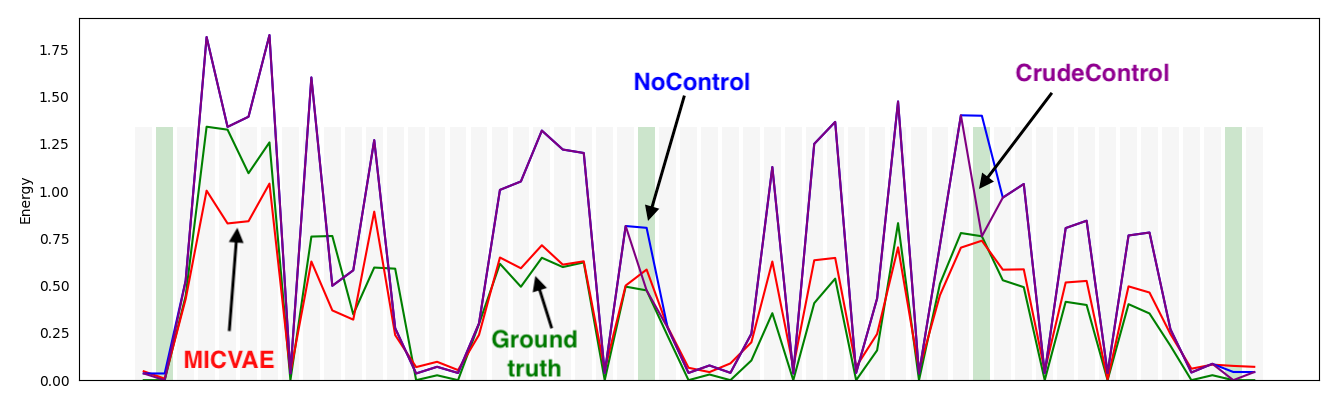
\includegraphics[width=\columnwidth]{figures/demo_a09_08q_004_energy.png}}
    \vskip -0.1in
    \caption{Our model produces plausible prosody, whereas Crude Control produces inconsistent prosody. The control points are shown with green vertical bars.} \crit{[Where is No Control? Show the time axis.]}
    \label{fig:demo}
    \vskip -5pt
\end{figure}

\begin{figure}[t]
    \centerline{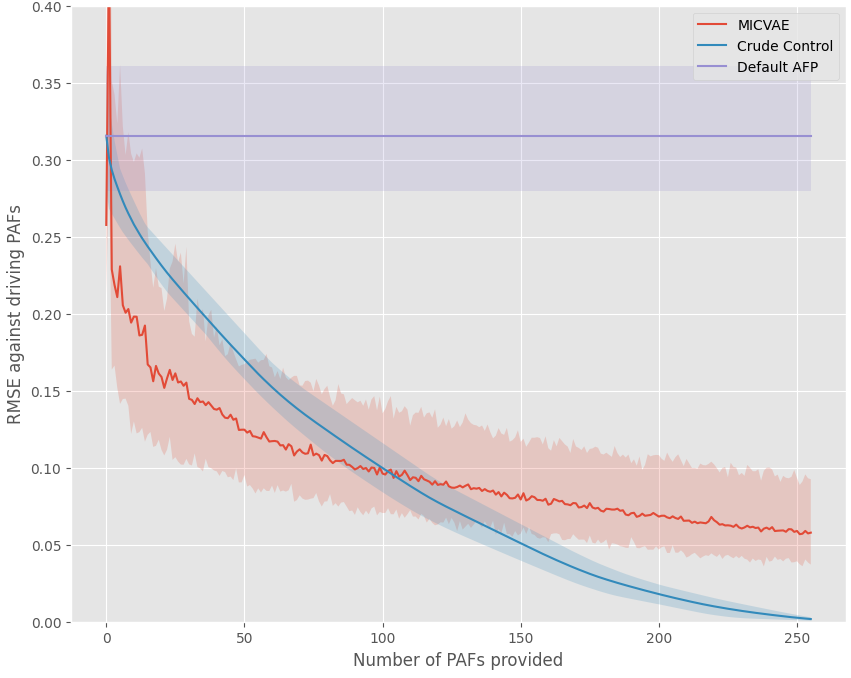
\includegraphics[width=\columnwidth]{figures/efficiency.pdf}}
    \vskip -0.15in
    \caption{Our model controls prosody efficiently. Its generated acoustic features are closer to the ground-truth rendition than is the manually modified output of the imputation model, called Crude-Control.}
    \label{fig:iterative}
    \vskip -0.2in
\end{figure}

In this section, I show that our model architecture (MIVAE) is a competent choice of architecture for this imputation task. I assess efficiency by how many control points are required for the model to produce outputs that align with the user's intention. Alignment is measured by the Root Mean Squared Error (RMSE) \crit{[Mean over what?]} between the generated and ground-truth acoustic features. We feed the model with additional control points from our test set \crit{[What is this test set? Is it the same as before?]} incrementally. In this ``iterative refinement'' process the acoustic feature with the highest RMSE in the previous generation is provided in the next step. A lower RMSE achieved with fewer input acoustic features directly translates to efficiency; it implies less user input is required to generate satisfactory prosodic instances.

Human \crit{[What is the loop?]} control is simulated by selecting a subset of acoustic features, referred to as control points, from one actor's rendition of a given test sentence. \crit{[What's the control point, the subset? What does it mean to get the control points from the speaker rather than a human user?]} These control points condition our acoustic feature Predictor (AFP) model, with the remaining acoustic features being generated by the model. We use Root Mean Square Error (RMSE) to quantify the quality of control between model-generated and ground-truth acoustic features. \crit{[This is only relevant for iterative refinement.]}

The model is conditioned on control points from one actor (control speaker) but uses the speaker label \crit{[What is the speaker label?]} from another actor (target speaker). This ensures that the control is attributable to the control points rather than the speaker label~\citep{siniIntroducingProsodicSpeaker2020}.

Our experiments aim to adapt to different prosody values during test time while controlling for possible confounds from speaker identity. To address this confound, we randomize speakers, which also happens to correspond to speaker adaptation. \crit{[What is this?]} By performing per-speaker acoustic feature normalization, the effect of speaker identity is primarily reflected in the relationship between prosody and text, rather than the density of prosody itself. \crit{[Expand explanation. I don't follow. What does it mean to be a confound in the test set. We switch speaker labels basically for ablation rather than the ultimate evaluation.]}

It is important to note that, in the context of speaker adaptation, we do not explicitly focus on speaker similarity since we are dealing with vanilla TTS (with control). This implies that the test speaker must be included in the training dataset. Consequently, we do not conduct speaker similarity tests, which would be a necessary aspect of speaker adaptation research.

We use this automated evaluation to (a) ensure that the experiments are reproducible and (b) enable larger scale experiments which would be costly to run using with humans.

\paragraph{Baselines.} I use the following baselines to show the efficiency of MIVAE as a control method.

\begin{enumerate}
    \item No-Control. The default prosody model: predicts acoustic features from phonemes, speaker identity, and style code. Uses the same decoder architecture as the MIVAE. \crit{[Where have you described this before?]}
    \item Crude Control. A na\"ive system that forcefully modifies predicted values individually, this straw-man represents a controllable model that is entirely inconsistent. Its default prosody is generated with No-Control, and then modified manually with the control points\footnote{Samples demonstrating TTS for these systems can be found here, \href{https://anonymous-submission-563098.github.io/sparse-control/}{anonymous-submission-563098.github.io/sparse-control}}.
\end{enumerate}

\crit{[These baselines are missing a sense of necessary inevitability. Why are we forced to use these baselines? Why Masked CVAE rather than an earlier baseline? It doesn't make sense to put baselines here, they belong to the whole chapter. Unless we are talking about ablation.]}

% In order to justify our choice of architecture, and to show that our model is relatively competent, we also compare against a conditional variational autoencoder trained with masking, and the conditional variational autoencoder not conditioned on partial inputs, but with the output modified to match the correct values (crude control).

% \paragraph{Masked CVAE} \crit{[This is answering a question that no one asked.]} Masked CVAE is a baseline system that uses the standard approach of masking for missing data imputation and inpainting~\citep{elharroussImageInpaintingReview2020} \crit{[Are these separate tasks?]}. Masked CVAE has a similar architecture to MIVAE. The primary difference lies in the encoder design. Masked CVAE employs a multi-layer Recurrent Neural Network (RNN) as its encoder. Input acoustic features are augmented with an additional binary instance for each of the three streams ($F_0$, energy, duration) to indicate whether a given acoustic feature is provided (a) or missing (0). Unlike MIVAE, which is inherently robust to varying levels of input missingness, Masked CVAE must be trained with fixed sparsity in order to learn what the values 0,1 in the mask denote. During training, a fixed missingness percentage $ P $ is set, and $ P \% $ of the acoustic features are randomly masked out for each training sentence.

% However, masked CVAE is not invariant to the number of control points like MIVAE is, so it generalises poorly to patterns of missingness unseen during training. \crit{[Why? Why does number of points equate to patterns of missingness.]}

\crit{[Why is the Bernoulli transformer not included here? That's the main baseline.]}

\subsection{Results}

\crit{[One output is eyeballing. Several outputs mean a robust conclusion.]}

Figure~\ref{fig:iterative} reveals that MIVAE significantly outperforms the Crude-Control method, achieving lower RMSEs across a realistic range of missingness (between 4 and 70 acoustic features). Our model (MIVAE) produces prosody closer to the ground-truth than the prosody resulting from manually setting the output acoustic features to default values, meaning MIVAE uses the learned structure of prosody data to fill in the gaps between the control points. The fact that Crude Control performs better than MIVAE is to be expected when the missingness rate approaches 0, because we are manually switching all acoustic features to the values extracted from the ground-truth utterance.

% As illustrated in Figure~\ref{fig:robustness}, MIVAE outperforms all versions of Masked CVAE, even with the same model capacity. The results indicate that Masked CVAEs fail to adapt to varying missingness patterns effectively, emphasizing the robustness of MIVAE. Note that our evaluation results generalise to other generative models than CVAE.\@ We compare different conditioning mechanisms (multiple-instance vs masking) rather than different generator architectures.

\subsection{Downstream performance}

\begin{figure}
    \begin{center}
    \centerline{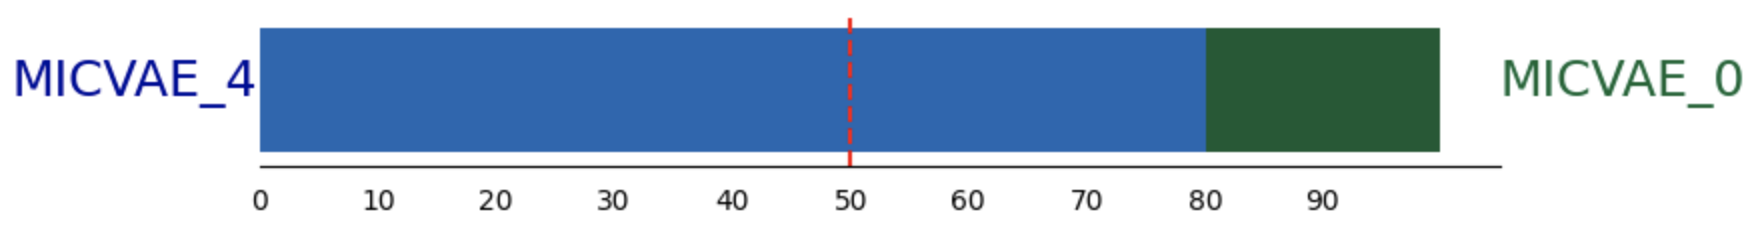
\includegraphics[width=\columnwidth]{figures/faithfulness.png}}
    \vskip -0.15in
    \caption{4 control points are enough to bring our model's output significantly closer to the reference utterance. These are ratings in an A/B test where the question is ``Which of these is closer to the reference ground-truth control audio?''.} \crit{[Do you need a figure to show one number?]}
    \label{fig:faithfulness}
    \end{center}
    \vskip -0.3in
\end{figure}

I also demonstrate the efficiency of MIVAE as a prosody control method by running a subjective listening test. I conduct an A/B listening test involving 20 native Latin American Spanish speakers. Participants choose which of two audio outputs (one with 4 input acoustic features and one with 0) sounds closer to a reference ground-truth audio. We chose 4 and 0 to demonstrate the impact that just 4 control points can have on the prosody.

Speech is synthesized using a TTS system conditioned on MIVAE's acoustic features. The system includes a Latin American Spanish front-end for text normalization and grapheme-to-phoneme conversion. The acoustic model relies on Ctrl-P~\citep{mohanCtrlPTemporalControl2021}, an attention-based Tacotron-2 variant, while the neural vocoder is WaveRNN~\citep{vandenoordWaveNetGenerativeModel2016}. \crit{[Who cares about this? Is it relevant?]}

Figure~\ref{fig:faithfulness} reveals that MIVAE with 4 input acoustic features is significantly perceived as closer to the reference audio compared to the version without any input acoustic features. This not only confirms the model's faithfulness to user intentions but also underscores its efficiency, as it achieves these results with a minimum number of input acoustic features.



\section{Conclusion}

This chapter introduced a new problem formulation for missing data imputation called versatile imputation. This formulation reflects the common real-world setting where models trained on complete data are deployed for imputation under unknown missingness patterns. Existing deep learning methods generalise poorly to unseen patterns of missingness. To address this limitation, I proposed a novel method, the Multiple-Instance Variational Autoencoder (MIVAE), leveraging the group-instance model to encourage maximum information extraction from individual data instances. Evaluation on the task of prosody control for text-to-speech synthesis demonstrated that MIVAE generalises significantly better to unseen missingness densities compared to conventional masked autoencoder methods. Moreover, the proposed model efficiently controls prosody, requiring minimal user input to achieve accurate imputation. These results suggest that MIVAE provides a promising direction for tackling versatile imputation in a range of high-dimensional data domains.

\biblio

\end{document}
